\documentclass[10pt,twocolumn]{article}
\usepackage[T1]{fontenc}
\usepackage[utf8]{inputenc}
\usepackage[margin=0.75in,columnsep=0.25in]{geometry}
\usepackage{booktabs}
\usepackage{graphicx}
\usepackage{longtable}
\usepackage{pdflscape}
\usepackage{pgfplots}
\pgfplotsset{compat=1.18}
\usetikzlibrary{positioning,arrows.meta}
\usepackage{microtype}
\setlength{\tabcolsep}{4pt}
\renewcommand{\topfraction}{0.9}
\renewcommand{\dbltopfraction}{0.9}
\renewcommand{\textfraction}{0.1}
\renewcommand{\floatpagefraction}{0.7}
\renewcommand{\dblfloatpagefraction}{0.7}
\setcounter{topnumber}{3}
\setcounter{dbltopnumber}{3}
\setcounter{totalnumber}{5}
\usepackage[round,authoryear]{natbib}
\usepackage{url}
\usepackage[hidelinks]{hyperref}
\usepackage{doi}
\usepackage{orcidlink}
\hypersetup{pdftitle={OpenCloudModel Regions: An Evidence-Linked Dataset of Cloud Region Locations and Codes},pdfauthor={Andrew Broekman},pdfkeywords={cloud regions, location codes, IATA, UN/LOCODE, data provenance}}
\newcommand{\candidateCount}{7}
\newcommand{\feedRegions}{19}
\newcommand{\feedConflicts}{4}
\newcommand{\regionCount}{380}
\newcommand{\providerCount}{13}
\newcommand{\placeCount}{141}
\newcommand{\evidenceCount}{870}
\newcommand{\curatedEvidenceCount}{266}
\newcommand{\callCount}{304}
\newcommand{\highCallCount}{18}
\newcommand{\tableDiffCount}{175}
\newcommand{\airportRegions}{379}
\newcommand{\metroRegions}{138}
\newcommand{\metroDistinct}{21}
\newcommand{\locodeRegions}{370}
\newcommand{\clliRegions}{138}
\newcommand{\tableADistinct}{131}
\newcommand{\tableBDistinct}{105}
\newcommand{\tableCDistinct}{125}
\newcommand{\tableDiffAC}{134}
\newcommand{\tableDiffBC}{41}
\newcommand{\gradeVendorStated}{335}
\newcommand{\gradeAssumed}{1}
\newcommand{\documentCount}{474}
\newcommand{\documentPublic}{441}
\newcommand{\documentRestricted}{33}
\newcommand{\gradeVendorDocument}{11}
\newcommand{\gradePublicRecord}{5}
\newcommand{\gradeReported}{1}
\newcommand{\gradePartial}{8}
\newcommand{\gradeNetwork}{0}
\newcommand{\precisionCity}{335}
\newcommand{\precisionCoarse}{44}
\newcommand{\metroOrAirportDistinct}{119}
\newcommand{\excludedCount}{20}
\newcommand{\verifyTotal}{487}
\newcommand{\verifyFound}{436}
\newcommand{\verifySaved}{49}
\newcommand{\verifyNoQuote}{0}
\newcommand{\verifyShort}{22}
\newcommand{\verifyNotFound}{2}
\newcommand{\placedByDocument}{16}
\newcommand{\placedByMemory}{4}
\newcommand{\placedNone}{1}
\newcommand{\verifyFormat}{0}
\newcommand{\verifyUnreachable}{0}

\newcommand{\capUsed}{90}
\newcommand{\capSelected}{90}
\newcommand{\capLow}{84}
\newcommand{\capHigh}{102.5}
\newcommand{\capMidpoint}{93}
\newcommand{\capPeak}{84.1}
\newcommand{\capRegions}{379}
\newcommand{\capCount}{64}
\newcommand{\capRadius}{100}
\newcommand{\capSharedAt}{319}
\newcommand{\capSharedA}{310}
\newcommand{\capSharedB}{338}
\newcommand{\capRecallAt}{91.0}
\newcommand{\capRecallA}{84.4}
\newcommand{\capRecallMax}{91.7}
\newcommand{\capFalseAt}{5}
\newcommand{\capFalseB}{135}
\newcommand{\capMaxAt}{110}
\newcommand{\capMaxB}{193}
\newcommand{\capBootLow}{59}
\newcommand{\capBootHigh}{122}
\newcommand{\capMovedCount}{41}
\newcommand{\capSplits}{86}
\newcommand{\capBorderSplits}{79}
\newcommand{\capOtherSplits}{7}
\newcommand{\capMixedGood}{6}
\newcommand{\capMixedBad}{30}
\newcommand{\capMixedLow}{100}
\newcommand{\capMixedHigh}{125}
\newcommand{\metroLinks}{610}
\newcommand{\metroNinetyFive}{62}
\newcommand{\metroNinetyNine}{124}
\newcommand{\capRuleRuns}{200}
\newcommand{\capRuleShare}{54}
\newcommand{\capRuleLow}{70}
\newcommand{\capRuleMedian}{90}
\newcommand{\capRuleHigh}{130}
\newcommand{\capRuleKept}{11}
\newcommand{\capRuleVendors}{13}
\newcommand{\capRuleMoved}{Alibaba 110~km and Huawei 110~km}
\newcommand{\capIntervalLow}{84}
\newcommand{\capIntervalHigh}{102.5}
\newcommand{\capIntervalPairs}{870}
\newcommand{\capIntervalFalse}{5}
\newcommand{\capUpperMedian}{102}
\newcommand{\capUpperLow}{102}
\newcommand{\capUpperHigh}{122}
\newcommand{\capLowerMedian}{84}
\newcommand{\capLowerLow}{53}
\newcommand{\capLowerHigh}{84}
\newcommand{\capCityShare}{26}
\newcommand{\capCityMedian}{90}
\newcommand{\capCityLow}{29}
\newcommand{\capCityHigh}{140}
\newcommand{\capCityUpperMedian}{111}
\newcommand{\capCityUpperLow}{102}
\newcommand{\capCityUpperHigh}{123}
\newcommand{\capCityLowerMedian}{53}
\newcommand{\capCityLowerLow}{0}
\newcommand{\capCityLowerHigh}{122}
\newcommand{\capCityInside}{57}
\newcommand{\capRegionInside}{63}
\newcommand{\capRegionHolds}{96}
\newcommand{\capCityHolds}{93}

\newcommand{\placerRegions}{380}
\newcommand{\placerPlaced}{371}
\newcommand{\placerAbstained}{9}
\newcommand{\placerAccuracy}{98.4}
\newcommand{\placerHoldoutRegions}{121}
\newcommand{\placerHoldoutPlaced}{116}
\newcommand{\placerHoldoutAccuracy}{96.6}
\newcommand{\placerDevAccuracy}{99.2}
\newcommand{\placerAgreedRegions}{188}
\newcommand{\placerAgreedMatched}{188}
\newcommand{\placerOverturnedTotal}{7}
\newcommand{\placerOverturnedFlagged}{7}
\newcommand{\placerOverturnedAccepted}{0}
\newcommand{\placerOverturnedMatching}{0}
\newcommand{\placerHoldoutLow}{91.5}
\newcommand{\placerHoldoutHigh}{98.7}
\newcommand{\placerAllLow}{96.5}
\newcommand{\placerAllHigh}{99.3}

\newcommand{\llmRulesAnswered}{371}
\newcommand{\llmRulesMatched}{365}
\newcommand{\llmRulesRegions}{380}
\newcommand{\llmRulesRescued}{0}
\newcommand{\llmRulesFromPassage}{0}
\newcommand{\llmRulesUnsupported}{0}
\newcommand{\llmRulesUnresolved}{0}
\newcommand{\llmRulesHoldoutAnswered}{116}
\newcommand{\llmRulesHoldoutMatched}{112}
\newcommand{\llmRulesReviewAnswered}{40}
\newcommand{\llmRulesReviewMatched}{38}
\newcommand{\llmRulesReviewRegions}{49}
\newcommand{\llmRulesTurnedMatched}{3}
\newcommand{\llmRulesTurnedAnswered}{5}
\newcommand{\llmRulesTurnedRegions}{7}
\newcommand{\llmLabelAnswered}{333}
\newcommand{\llmLabelMatched}{329}
\newcommand{\llmLabelRegions}{380}
\newcommand{\llmLabelRescued}{0}
\newcommand{\llmLabelFromPassage}{0}
\newcommand{\llmLabelUnsupported}{0}
\newcommand{\llmLabelUnresolved}{10}
\newcommand{\llmLabelHoldoutAnswered}{107}
\newcommand{\llmLabelHoldoutMatched}{104}
\newcommand{\llmLabelReviewAnswered}{4}
\newcommand{\llmLabelReviewMatched}{4}
\newcommand{\llmLabelReviewRegions}{49}
\newcommand{\llmLabelTurnedMatched}{0}
\newcommand{\llmLabelTurnedAnswered}{0}
\newcommand{\llmLabelTurnedRegions}{7}
\newcommand{\llmMemoryAnswered}{363}
\newcommand{\llmMemoryMatched}{348}
\newcommand{\llmMemoryRegions}{380}
\newcommand{\llmMemoryRescued}{4}
\newcommand{\llmMemoryFromPassage}{0}
\newcommand{\llmMemoryUnsupported}{0}
\newcommand{\llmMemoryUnresolved}{3}
\newcommand{\llmMemoryHoldoutAnswered}{116}
\newcommand{\llmMemoryHoldoutMatched}{110}
\newcommand{\llmMemoryReviewAnswered}{32}
\newcommand{\llmMemoryReviewMatched}{21}
\newcommand{\llmMemoryReviewRegions}{49}
\newcommand{\llmMemoryTurnedMatched}{3}
\newcommand{\llmMemoryTurnedAnswered}{4}
\newcommand{\llmMemoryTurnedRegions}{7}
\newcommand{\llmRagAnswered}{321}
\newcommand{\llmRagMatched}{317}
\newcommand{\llmRagRegions}{380}
\newcommand{\llmRagRescued}{5}
\newcommand{\llmRagFromPassage}{321}
\newcommand{\llmRagUnsupported}{1}
\newcommand{\llmRagUnresolved}{15}
\newcommand{\llmRagHoldoutAnswered}{101}
\newcommand{\llmRagHoldoutMatched}{101}
\newcommand{\llmRagReviewAnswered}{29}
\newcommand{\llmRagReviewMatched}{27}
\newcommand{\llmRagReviewRegions}{49}
\newcommand{\llmRagTurnedMatched}{4}
\newcommand{\llmRagTurnedAnswered}{4}
\newcommand{\llmRagTurnedRegions}{7}

\newcommand{\mutationControl}{265}
\newcommand{\mutationControlTotal}{266}
\newcommand{\mutationQuoteRecords}{265}
\newcommand{\mutationQuoteFalse}{2}
\newcommand{\mutationQuoteShare}{0.8}
\newcommand{\mutationQuoteLow}{0.2}
\newcommand{\mutationQuoteHigh}{2.7}
\newcommand{\mutationCityRecords}{254}
\newcommand{\mutationCityFalse}{1}
\newcommand{\mutationCityShare}{0.4}
\newcommand{\mutationCityLow}{0.1}
\newcommand{\mutationCityHigh}{2.2}
\newcommand{\mutationShortFalse}{1}
\newcommand{\mutationShortRecords}{27}
\newcommand{\mutationLongFalse}{0}
\newcommand{\mutationLongRecords}{80}
\newcommand{\extractTraditionalAnswered}{207}
\newcommand{\extractTraditionalMatched}{121}
\newcommand{\extractTraditionalLow}{52}
\newcommand{\extractTraditionalHigh}{65}
\newcommand{\extractStatisticalAnswered}{207}
\newcommand{\extractStatisticalMatched}{127}
\newcommand{\extractStatisticalLow}{55}
\newcommand{\extractStatisticalHigh}{68}
\newcommand{\extractRagAnswered}{321}
\newcommand{\extractRagMatched}{317}
\newcommand{\extractRagLow}{97}
\newcommand{\extractRagHigh}{100}
\newcommand{\extractRagQwenSixAnswered}{313}
\newcommand{\extractRagQwenSixMatched}{305}
\newcommand{\extractRagQwenSixLow}{95}
\newcommand{\extractRagQwenSixHigh}{99}
\newcommand{\extractRagGlmAnswered}{313}
\newcommand{\extractRagGlmMatched}{303}
\newcommand{\extractRagGlmLow}{94}
\newcommand{\extractRagGlmHigh}{98}
\newcommand{\extractLabelAnswered}{333}
\newcommand{\extractLabelMatched}{329}
\newcommand{\extractLabelLow}{97}
\newcommand{\extractLabelHigh}{100}
\newcommand{\areaRiskSafe}{6}
\newcommand{\areaRiskAtRisk}{3}
\newcommand{\corpusDocuments}{474}
\newcommand{\corpusFetched}{441}
\newcommand{\modelGainRegions}{7}
\newcommand{\vendorDocWithModel}{11}
\newcommand{\vendorDocWithoutModel}{4}

\newcommand{\statRulesVsRagP}{<0.001}
\newcommand{\statRulesVsRagHolm}{<0.001}
\newcommand{\statRulesVsRagOnlyFirst}{53}
\newcommand{\statRulesVsRagOnlySecond}{5}
\newcommand{\statRulesVsMemoryP}{<0.001}
\newcommand{\statRulesVsMemoryHolm}{0.006}
\newcommand{\statRulesVsMemoryOnlyFirst}{21}
\newcommand{\statRulesVsMemoryOnlySecond}{4}
\newcommand{\statRulesVsLabelP}{<0.001}
\newcommand{\statRulesVsLabelHolm}{<0.001}
\newcommand{\statRulesVsLabelOnlyFirst}{36}
\newcommand{\statRulesVsLabelOnlySecond}{0}
\newcommand{\statRulesVsRagQwenthreeSixP}{<0.001}
\newcommand{\statRulesVsRagQwenthreeSixHolm}{<0.001}
\newcommand{\statRulesVsRagQwenthreeSixOnlyFirst}{65}
\newcommand{\statRulesVsRagQwenthreeSixOnlySecond}{5}
\newcommand{\statRulesVsRagGlmFourSevenP}{<0.001}
\newcommand{\statRulesVsRagGlmFourSevenHolm}{<0.001}
\newcommand{\statRulesVsRagGlmFourSevenOnlyFirst}{67}
\newcommand{\statRulesVsRagGlmFourSevenOnlySecond}{5}
\newcommand{\statRagVsMemoryP}{<0.001}
\newcommand{\statRagVsMemoryHolm}{<0.001}
\newcommand{\statRagVsMemoryOnlyFirst}{13}
\newcommand{\statRagVsMemoryOnlySecond}{44}
\newcommand{\statRagVsLabelP}{0.169}
\newcommand{\statRagVsLabelHolm}{0.337}
\newcommand{\statRagVsLabelOnlyFirst}{26}
\newcommand{\statRagVsLabelOnlySecond}{38}
\newcommand{\statRagVsRagQwenthreeSixP}{0.036}
\newcommand{\statRagVsRagQwenthreeSixHolm}{0.107}
\newcommand{\statRagVsRagQwenthreeSixOnlyFirst}{20}
\newcommand{\statRagVsRagQwenthreeSixOnlySecond}{8}
\newcommand{\statRagVsRagGlmFourSevenP}{0.016}
\newcommand{\statRagVsRagGlmFourSevenHolm}{0.064}
\newcommand{\statRagVsRagGlmFourSevenOnlyFirst}{22}
\newcommand{\statRagVsRagGlmFourSevenOnlySecond}{8}
\newcommand{\statMemoryVsLabelP}{<0.001}
\newcommand{\statMemoryVsLabelHolm}{<0.001}
\newcommand{\statMemoryVsLabelOnlyFirst}{19}
\newcommand{\statMemoryVsLabelOnlySecond}{0}
\newcommand{\statMemoryVsRagQwenthreeSixP}{<0.001}
\newcommand{\statMemoryVsRagQwenthreeSixHolm}{<0.001}
\newcommand{\statMemoryVsRagQwenthreeSixOnlyFirst}{56}
\newcommand{\statMemoryVsRagQwenthreeSixOnlySecond}{13}
\newcommand{\statMemoryVsRagGlmFourSevenP}{<0.001}
\newcommand{\statMemoryVsRagGlmFourSevenHolm}{<0.001}
\newcommand{\statMemoryVsRagGlmFourSevenOnlyFirst}{58}
\newcommand{\statMemoryVsRagGlmFourSevenOnlySecond}{13}
\newcommand{\statLabelVsRagQwenthreeSixP}{0.005}
\newcommand{\statLabelVsRagQwenthreeSixHolm}{0.025}
\newcommand{\statLabelVsRagQwenthreeSixOnlyFirst}{46}
\newcommand{\statLabelVsRagQwenthreeSixOnlySecond}{22}
\newcommand{\statLabelVsRagGlmFourSevenP}{0.004}
\newcommand{\statLabelVsRagGlmFourSevenHolm}{0.023}
\newcommand{\statLabelVsRagGlmFourSevenOnlyFirst}{51}
\newcommand{\statLabelVsRagGlmFourSevenOnlySecond}{25}
\newcommand{\statRagQwenthreeSixVsRagGlmFourSevenP}{0.868}
\newcommand{\statRagQwenthreeSixVsRagGlmFourSevenHolm}{0.868}
\newcommand{\statRagQwenthreeSixVsRagGlmFourSevenOnlyFirst}{19}
\newcommand{\statRagQwenthreeSixVsRagGlmFourSevenOnlySecond}{17}
\newcommand{\statRulesVsRagAnsweredP}{1.000}
\newcommand{\statRulesVsRagAnsweredHolm}{1.000}
\newcommand{\statRulesVsRagAnsweredPairs}{318}
\newcommand{\statRulesVsRagAnsweredOnlyFirst}{3}
\newcommand{\statRulesVsRagAnsweredOnlySecond}{2}
\newcommand{\statRulesVsMemoryAnsweredP}{0.016}
\newcommand{\statRulesVsMemoryAnsweredHolm}{0.234}
\newcommand{\statRulesVsMemoryAnsweredPairs}{356}
\newcommand{\statRulesVsMemoryAnsweredOnlyFirst}{7}
\newcommand{\statRulesVsMemoryAnsweredOnlySecond}{0}
\newcommand{\statRulesVsLabelAnsweredP}{1.000}
\newcommand{\statRulesVsLabelAnsweredHolm}{1.000}
\newcommand{\statRulesVsLabelAnsweredPairs}{333}
\newcommand{\statRulesVsLabelAnsweredOnlyFirst}{0}
\newcommand{\statRulesVsLabelAnsweredOnlySecond}{0}
\newcommand{\statRulesVsRagQwenthreeSixAnsweredP}{0.344}
\newcommand{\statRulesVsRagQwenthreeSixAnsweredHolm}{1.000}
\newcommand{\statRulesVsRagQwenthreeSixAnsweredPairs}{311}
\newcommand{\statRulesVsRagQwenthreeSixAnsweredOnlyFirst}{7}
\newcommand{\statRulesVsRagQwenthreeSixAnsweredOnlySecond}{3}
\newcommand{\statRulesVsRagGlmFourSevenAnsweredP}{0.227}
\newcommand{\statRulesVsRagGlmFourSevenAnsweredHolm}{1.000}
\newcommand{\statRulesVsRagGlmFourSevenAnsweredPairs}{310}
\newcommand{\statRulesVsRagGlmFourSevenAnsweredOnlyFirst}{8}
\newcommand{\statRulesVsRagGlmFourSevenAnsweredOnlySecond}{3}
\newcommand{\statRagVsMemoryAnsweredP}{0.070}
\newcommand{\statRagVsMemoryAnsweredHolm}{0.984}
\newcommand{\statRagVsMemoryAnsweredPairs}{314}
\newcommand{\statRagVsMemoryAnsweredOnlyFirst}{7}
\newcommand{\statRagVsMemoryAnsweredOnlySecond}{1}
\newcommand{\statRagVsLabelAnsweredP}{1.000}
\newcommand{\statRagVsLabelAnsweredHolm}{1.000}
\newcommand{\statRagVsLabelAnsweredPairs}{294}
\newcommand{\statRagVsLabelAnsweredOnlyFirst}{1}
\newcommand{\statRagVsLabelAnsweredOnlySecond}{1}
\newcommand{\statRagVsRagQwenthreeSixAnsweredP}{0.219}
\newcommand{\statRagVsRagQwenthreeSixAnsweredHolm}{1.000}
\newcommand{\statRagVsRagQwenthreeSixAnsweredPairs}{304}
\newcommand{\statRagVsRagQwenthreeSixAnsweredOnlyFirst}{5}
\newcommand{\statRagVsRagQwenthreeSixAnsweredOnlySecond}{1}
\newcommand{\statRagVsRagGlmFourSevenAnsweredP}{0.688}
\newcommand{\statRagVsRagGlmFourSevenAnsweredHolm}{1.000}
\newcommand{\statRagVsRagGlmFourSevenAnsweredPairs}{303}
\newcommand{\statRagVsRagGlmFourSevenAnsweredOnlyFirst}{4}
\newcommand{\statRagVsRagGlmFourSevenAnsweredOnlySecond}{2}
\newcommand{\statMemoryVsLabelAnsweredP}{1.000}
\newcommand{\statMemoryVsLabelAnsweredHolm}{1.000}
\newcommand{\statMemoryVsLabelAnsweredPairs}{333}
\newcommand{\statMemoryVsLabelAnsweredOnlyFirst}{0}
\newcommand{\statMemoryVsLabelAnsweredOnlySecond}{0}
\newcommand{\statMemoryVsRagQwenthreeSixAnsweredP}{1.000}
\newcommand{\statMemoryVsRagQwenthreeSixAnsweredHolm}{1.000}
\newcommand{\statMemoryVsRagQwenthreeSixAnsweredPairs}{306}
\newcommand{\statMemoryVsRagQwenthreeSixAnsweredOnlyFirst}{6}
\newcommand{\statMemoryVsRagQwenthreeSixAnsweredOnlySecond}{7}
\newcommand{\statMemoryVsRagGlmFourSevenAnsweredP}{0.227}
\newcommand{\statMemoryVsRagGlmFourSevenAnsweredHolm}{1.000}
\newcommand{\statMemoryVsRagGlmFourSevenAnsweredPairs}{304}
\newcommand{\statMemoryVsRagGlmFourSevenAnsweredOnlyFirst}{3}
\newcommand{\statMemoryVsRagGlmFourSevenAnsweredOnlySecond}{8}
\newcommand{\statLabelVsRagQwenthreeSixAnsweredP}{0.289}
\newcommand{\statLabelVsRagQwenthreeSixAnsweredHolm}{1.000}
\newcommand{\statLabelVsRagQwenthreeSixAnsweredPairs}{292}
\newcommand{\statLabelVsRagQwenthreeSixAnsweredOnlyFirst}{6}
\newcommand{\statLabelVsRagQwenthreeSixAnsweredOnlySecond}{2}
\newcommand{\statLabelVsRagGlmFourSevenAnsweredP}{1.000}
\newcommand{\statLabelVsRagGlmFourSevenAnsweredHolm}{1.000}
\newcommand{\statLabelVsRagGlmFourSevenAnsweredPairs}{284}
\newcommand{\statLabelVsRagGlmFourSevenAnsweredOnlyFirst}{3}
\newcommand{\statLabelVsRagGlmFourSevenAnsweredOnlySecond}{2}
\newcommand{\statRagQwenthreeSixVsRagGlmFourSevenAnsweredP}{1.000}
\newcommand{\statRagQwenthreeSixVsRagGlmFourSevenAnsweredHolm}{1.000}
\newcommand{\statRagQwenthreeSixVsRagGlmFourSevenAnsweredPairs}{296}
\newcommand{\statRagQwenthreeSixVsRagGlmFourSevenAnsweredOnlyFirst}{4}
\newcommand{\statRagQwenthreeSixVsRagGlmFourSevenAnsweredOnlySecond}{5}
\newcommand{\statRagAndMemoryKappa}{0.32}
\newcommand{\statRagAndMemoryAgree}{85.0}
\newcommand{\statRagAndLabelKappa}{0.34}
\newcommand{\statRagAndLabelAgree}{83.2}
\newcommand{\statRagAndRagQwenthreeSixKappa}{0.75}
\newcommand{\statRagAndRagQwenthreeSixAgree}{92.6}
\newcommand{\statRagAndRagGlmFourSevenKappa}{0.74}
\newcommand{\statRagAndRagGlmFourSevenAgree}{92.1}
\newcommand{\statMemoryAndLabelKappa}{0.74}
\newcommand{\statMemoryAndLabelAgree}{95.0}
\newcommand{\statMemoryAndRagQwenthreeSixKappa}{0.27}
\newcommand{\statMemoryAndRagQwenthreeSixAgree}{81.8}
\newcommand{\statMemoryAndRagGlmFourSevenKappa}{0.26}
\newcommand{\statMemoryAndRagGlmFourSevenAgree}{81.3}
\newcommand{\statLabelAndRagQwenthreeSixKappa}{0.36}
\newcommand{\statLabelAndRagQwenthreeSixAgree}{82.1}
\newcommand{\statLabelAndRagGlmFourSevenKappa}{0.29}
\newcommand{\statLabelAndRagGlmFourSevenAgree}{80.0}
\newcommand{\statRagQwenthreeSixAndRagGlmFourSevenKappa}{0.70}
\newcommand{\statRagQwenthreeSixAndRagGlmFourSevenAgree}{90.5}
\newcommand{\statRulesMedianKm}{0}
\newcommand{\statRulesPninezeroKm}{0}
\newcommand{\statRulesMisses}{6}
\newcommand{\statRulesMissMedianKm}{99}
\newcommand{\statRagMedianKm}{0}
\newcommand{\statRagPninezeroKm}{0}
\newcommand{\statRagMisses}{4}
\newcommand{\statRagMissMedianKm}{287}
\newcommand{\statMemoryMedianKm}{0}
\newcommand{\statMemoryPninezeroKm}{0}
\newcommand{\statMemoryMisses}{15}
\newcommand{\statMemoryMissMedianKm}{237}
\newcommand{\statLabelMedianKm}{0}
\newcommand{\statLabelPninezeroKm}{0}
\newcommand{\statLabelMisses}{4}
\newcommand{\statLabelMissMedianKm}{70}
\newcommand{\statRagQwenthreeSixMedianKm}{0}
\newcommand{\statRagQwenthreeSixPninezeroKm}{0}
\newcommand{\statRagQwenthreeSixMisses}{8}
\newcommand{\statRagQwenthreeSixMissMedianKm}{782}
\newcommand{\statRagGlmFourSevenMedianKm}{0}
\newcommand{\statRagGlmFourSevenPninezeroKm}{0}
\newcommand{\statRagGlmFourSevenMisses}{10}
\newcommand{\statRagGlmFourSevenMissMedianKm}{355}
\newcommand{\statAllAgree}{279}

\newcommand{\listsRetrieved}{5 to 14 November 2026}
\newcommand{\documentsRetrieved}{9 to 12 November 2026}
\newcommand{\datasetVersion}{1.0.0}

\newcommand{\outsidePlacesCompared}{94}
\newcommand{\outsidePlacesNear}{72}
\newcommand{\outsidePlacesWide}{75}
\newcommand{\outsidePlacesShare}{77}
\newcommand{\outsidePlacesLow}{67}
\newcommand{\outsidePlacesHigh}{84}
\newcommand{\outsidePlacesMedianKm}{4}
\newcommand{\outsidePlacesFar}{22}
\newcommand{\outsidePlacesFarStated}{13}
\newcommand{\outsidePlacesMissing}{7}
\newcommand{\outsidePlacesExtra}{45}
\newcommand{\operatorSites}{343}
\newcommand{\operatorSitesResolved}{329}
\newcommand{\operatorCodeIsAirport}{324}
\newcommand{\operatorNearest}{263}
\newcommand{\operatorNearestShare}{80}
\newcommand{\operatorMajorHub}{242}
\newcommand{\operatorMajorHubShare}{74}
\newcommand{\operatorNearbyHub}{284}
\newcommand{\operatorNearbyHubShare}{86}

\newcommand{\zenlayerRegions}{20}
\newcommand{\zenlayerRegionsPlaced}{20}
\newcommand{\zenlayerRegionsSameName}{19}
\newcommand{\zenlayerMemoryAnswered}{1}
\newcommand{\zenlayerMemoryNear}{1}
\newcommand{\fastlySites}{201}
\newcommand{\fastlyPlaced}{189}
\newcommand{\fastlyWithPoint}{189}
\newcommand{\fastlyNear}{177}
\newcommand{\fastlyNearShare}{94}
\newcommand{\fastlyCodeIsAirport}{148}
\newcommand{\fastlyNearest}{86}
\newcommand{\fastlyNearestShare}{46}
\newcommand{\fastlyMajorHub}{81}
\newcommand{\fastlyMajorHubShare}{43}
\newcommand{\fastlyNearbyHub}{89}
\newcommand{\fastlyNearbyHubShare}{47}
\newcommand{\zenlayerZonesSites}{58}
\newcommand{\zenlayerZonesPlaced}{54}
\newcommand{\zenlayerZonesWithPoint}{0}
\newcommand{\zenlayerZonesNear}{0}
\newcommand{\zenlayerZonesNearShare}{0}
\newcommand{\zenlayerZonesCodeIsAirport}{45}
\newcommand{\zenlayerZonesNearest}{32}
\newcommand{\zenlayerZonesNearestShare}{59}
\newcommand{\zenlayerZonesMajorHub}{42}
\newcommand{\zenlayerZonesMajorHubShare}{78}
\newcommand{\zenlayerZonesNearbyHub}{43}
\newcommand{\zenlayerZonesNearbyHubShare}{80}

\newcommand{\reviewRecords}{270}
\newcommand{\reviewCannotOpen}{0}
\newcommand{\reviewOpened}{270}
\newcommand{\reviewOnPage}{270}
\newcommand{\reviewAgree}{269}
\newcommand{\reviewDisagree}{1}
\newcommand{\reviewWithdrawn}{1}

\newcommand{\code}[1]{\texttt{#1}}

\title{OpenCloudModel Regions: An Evidence-Linked Dataset of Cloud Region Locations and Codes}
\author{Andrew Broekman~\orcidlink{0000-0003-0338-4567}\\Mosox Digital Ltd., United Kingdom\\\small\url{https://orcid.org/0000-0003-0338-4567}}
\date{November 2026}

\begin{document}
\sloppy
\twocolumn[\begin{@twocolumnfalse}
\maketitle

\begin{abstract}
Cloud computing is sold from regions: groups of data centres that each vendor names in its own way. Software that compares clouds, names resources or estimates the carbon cost of computing must know where each region is, yet many vendors do not say, and the mappings in public use rarely show their sources. Each study therefore builds its own table, and those tables cannot easily be checked against each other. Here we show that the \regionCount{} published regions of \providerCount{} vendors can be mapped to places and to standard location codes by script from a fixed list of documents that we chose. After that list, every step is code or a locally run language model with fixed settings, so the mapping replays without further human judgement. Each region carries its evidence, a grade and a stated precision. For \gradeVendorStated{} regions the vendor's own list names the city; the rest rely on weaker evidence, some are known only to a country, and \placedNone{} could not be placed. Two reasonable naming rules give different codes for \tableDiffCount{} regions, nearly half, so the rule must be stated with the code. The resulting dataset, OpenCloudModel Regions, gives cloud regions a shared, auditable naming and makes clear which locations are vendor claims rather than measurements.
\end{abstract}
\vspace{1em}
\end{@twocolumnfalse}]


\section{Introduction}

A cloud region identifier such as \code{us-east-1} or \code{westus2} tells a reader little about geography. Some vendors publish a city. Others publish a state, a country or only a marketing name. Anyone comparing vendors needs to join these identifiers to something geographic. Carbon accounting is one such use, since the emissions of a cloud workload depend on the grid where its region sits~\citep{dodge2022measuring,radovanovic2023carbon,sukprasert2024limitations}. Yet existing open mappings usually record the result without recording how it was reached. Researchers meet the same gap: one study notes that AWS data centre street addresses ``are not explicitly published by Amazon'', that the mapping of availability zones to locations ``is not known'', and takes site locations from press reports, a web directory and a leaked document~\citep{yeganeh2019how}.

This paper treats that join as a data provenance problem. We ask three questions. Which code scheme can name the most regions? How strong is the evidence for where each region is? And can the whole mapping be rebuilt, checked and challenged region by region?

Our contributions are:
\begin{itemize}
\item A taxonomy that separates a vendor region, the place it maps to, the codes for that place and the evidence behind the mapping (Section~\ref{sec:design}).
\item An evidence grade and a separate precision for each region, so that a label such as ``Ashburn'' is not mistaken for proof at city level.
\item A coverage comparison of IATA airport codes, IATA metropolitan codes, UN/LOCODE and CLLI across \regionCount{} regions (Section~\ref{sec:results}).
\item Three naming tables and a register of every gap and conflict, built by a script from a published list of document links and released as the OpenCloudModel Regions dataset.
\end{itemize}
Each part has precedents, described next. The combination is what is new.

\section{Related work}
\label{sec:related}

\paragraph{Geographic hints in names.} Rocketfuel inferred router locations from ISP naming conventions, including city codes~\citep{spring2002measuring}. DRoP built a dictionary from GeoNames, IATA, ICAO, UN/LOCODE and a small CLLI subset, and recorded that the CLLI database is proprietary~\citep{huffaker2014drop}. HLOC extracted hints from reverse DNS and tested them with latency measurements~\citep{scheitle2017hloc}. Hoiho learned per-suffix patterns from dictionaries of airport codes, place names, UN/LOCODE, CLLI prefixes and PeeringDB facilities, and is our closest methodological precedent~\citep{luckie2021learning}. These systems decode names that operators already chose. Our problem runs the other way: choosing a code for a region whose location may be undisclosed.

\paragraph{Region-to-place datasets.} The Green Software Foundation's real-time cloud dataset gives AWS, Azure and Google Cloud regions, with locations as reported by the provider, coordinates and grid zones~\citep{gsf_real_time_cloud}. Other open lists map regions to coordinates or country codes~\citep{dgl_cloud_regions,wilbur_mcp_cloud_regions,ipregistry_aws_regions,cloudregion_pypi}. Carbon research also depends on such mappings~\citep{sukprasert2024limitations}. TeleGeography sells metro-level cloud region data under licence~\citep{telegeography_geocoded_license}. Studies also build such tables for their own use. One study places 187 regions of six vendors through a city database~\citep{lehdonvirta2024compute}, CloudCast publishes 11 cross-vendor hubs~\citep{rotman2022cloudcast}, CATS combines a TeleGeography map, a geocoder and grid polygons for 140 sites~\citep{chen2026cats}, and another sources AWS sites from press and leaks~\citep{yeganeh2019how}. The need we argue from is this repeated rebuilding. The closest precedent for codes with evidence is \code{awsgo}, an MIT-licensed repository with UN/LOCODE for 18 Azure and 11 AWS regions, with reference links on its Azure rows, most of them secondary~\citep{grokify_awsgo}. So neither a mapping to place nor UN/LOCODE on regions is new. What is new is the combination: all three code families, across many vendors, with a grade, a precision and evidence on each row. To our knowledge, no published source combines these.

\paragraph{Infrastructure-as-code tools.} Terraform modules are where region names meet practice, and most stop at short names. Cloud Posse covers AWS~\citep{tf_cloudposse_utils}, Claranet and Microsoft's own module cover Azure~\citep{tf_claranet_regions,tf_avm_regions}, and one family of modules gives short codes for six vendors, one module each~\citep{tf_abbreviation}. One Google Cloud module adds a city and coordinates, with estimates marked only in source comments~\citep{tf_memes_region}, and some providers' data sources return a city or a display name for that vendor alone. The closest cross-vendor tool we found is a Python package, not a Terraform module, with coordinates for nine clouds and no source per row~\citep{cloud_regions_info}. None of these returns IATA, UN/LOCODE or CLLI codes or per-row evidence.

\paragraph{Vendor-neutral naming.} FOCUS defines a Region ID column assigned by the host provider~\citep{focus_region_id}, and Kubernetes defines a region label filled in by the provider~\citep{kubernetes_labels}. Both standardise the field and leave its value to the vendor.

\paragraph{Auditing stated locations.} Constraint-Based Geolocation turns delay into distance limits and a confidence region~\citep{gueye2006constraint}. One-third of 2{,}269 commercial proxies tested were definitely not in their advertised country~\citep{weinberg2018how}. GeoFINDR proposes checking a cloud instance's location with RIPE Atlas landmarks, though its test machine sat on a university campus, so it reports nothing about a real provider~\citep{ider2025geofindr}. One study measured a real service~\citep{gondree2013geolocation}: using PlanetLab landmarks, it placed data in Amazon S3's Northern California region within about 11{,}000~km$^2$ when nearby landmarks were included, which its authors describe as small enough to identify a state or service region. That tests one region of one vendor, and it was not designed to check a stated city. Methods have been evaluated on commercial clouds more widely than this suggests: one study reports results on four providers from US landmarks~\citep{biswal2015enhanced}, another covers 14 AWS regions~\citep{stephanow2017continuous}, taking AWS's labels as the truth, and CDGeB offers a measurement benchmark, also on AWS with AWS's labels~\citep{offer2023cdgeb}. These evaluate methods and do not set out to test whether vendors' stated locations are true. IGOD proposes choosing fewer landmarks to locate a data centre~\citep{jaiswal2015igod,jaiswal2016igod}. Its workshop version reports no results for a real provider and describes a test on Amazon S3 as future work.

\paragraph{PeeringDB.} PeeringDB records are often used in this area, with mixed support. Network records are mostly current~\citep{lodhi2014using}, yet a check of 152 networks found substantial missing facility links~\citep{giotsas2015mapping}. In our data, PeeringDB shows where a network peers. We never use it to establish where a region is hosted.

\section{Taxonomy design}
\label{sec:design}

\paragraph{Layers.} The taxonomy has three layers. A \emph{region} is an identifier published by a vendor. A \emph{place} is a geographic entity with coordinates and a stable identifier we assign, such as \code{us-va-ashburn}. \emph{Codes} are attributes of a place: IATA, UN/LOCODE, CLLI prefix and an optional metropolitan code. Keeping our own place identifier avoids depending on a scheme with gaps or unclear reuse terms.

\paragraph{Evidence grades.} Each region takes the strongest grade its evidence supports, in this order: \code{vendor-stated} (the vendor's region list names the place), \code{vendor-document}, \code{audit-document}, \code{public-record} (an audit list ties the region to a facility code, and a government record puts the same operator and code in the area), \code{measured} (reserved, as we have run no measurements), \code{vendor-feed}, \code{reported} (press, government or directory), \code{network-presence} (PeeringDB only), \code{partial} and \code{assumed}. These rules decide a grade. A source that names the region and ties it to an area keeps its grade, and precision records how coarse the area is. A source that shows only the vendor's presence in a place, without naming the region, is \code{partial} whatever its type, so a vendor fact sheet naming a site in a state with one region is \code{partial}, because the link to the region is an inference. Any source we could not open is also \code{partial}, as is any collected record whose quote fails the check in Section~\ref{sec:method}. A vendor feed supports an area and never moves a place. A source that contradicts the placement grades only itself, as \code{assumed}. It does not lower the region's grade, and it raises a call for a person to read instead.

\paragraph{Precision.} Grade says how strong the source is. Precision says how fine it is: \code{city} when the vendor's label names a city, and \code{metro} otherwise. A rule sets it, so a label such as ``Ashburn'' on a region the vendor describes only as Virginia carries metro precision.

\paragraph{Evidence records.} Each record holds the claim, value, source type, publisher, URL, verbatim quote, stance and a note, following W3C PROV~\citep{w3c2013provdm} and the FAIR principle of detailed provenance~\citep{wilkinson2016fair}. The build exports this chain in PROV-O~\citep{w3c2013provo} as \code{output/provenance.jsonld}: each placement derives from its evidence records, each record names the document it quotes and the step that made it, and each step names the code digest, the model build and the frozen prompt it used. The file parses as RDF; we have not checked it against the PROV constraints. An RO-Crate description~\citep{soilandreyes2022rocrate} and a citation file~\citep{cff_format} describe the dataset as a whole.

\paragraph{Calls.} The build raises a call for every gap or doubt: no code available, a place resting on weak evidence, sources in conflict, two tables disagreeing, an airport serving several towns, or a vendor code that is really another airport's. Each call has a severity, and calls are published as data rather than resolved silently.

\paragraph{Three naming tables.} Resource names commonly need a short code, and three letters are the constraint we started from. The \emph{nearest-airport} table takes the nearest scheduled large or medium airport in the same country, using OurAirports~\citep{ourairports_data}. The \emph{major-hub} table takes the best-connected such airport in the same country within 200~km, by OpenTravelData page rank~\citep{opentraveldata}. Page rank is not passenger traffic, and 200~km is a parameter we set. A major hub must be in the region's own country. A code shared across a border would hide differences in law and data residency, so we accept the lower overlap. The \emph{nearby-hub} table uses the major hub when it is within the cap, \capUsed{}~km, of the region and the nearest airport otherwise; Section~\ref{sec:cap} explains how code selects the cap. All three append a number when one vendor has several regions on a code (\code{iad}, \code{iad2}). Assigned codes live in an append-only register, so a new region cannot renumber an existing one.

\paragraph{Released files.} Table~\ref{tab:files} lists the main files of the dataset. Each is plain CSV or JSON, and \code{README.md} describes them.

\begin{table}[t]
\centering
\small
\begin{tabular}{p{0.41\columnwidth}p{0.51\columnwidth}}
\toprule
File & Contents \\
\midrule
\code{output/\allowbreak regions.csv} & One row for each of the \regionCount{} regions: vendor, region ID and name, place, coordinates, grade, precision, the three codes with the reason for each, the class of the nearby hub's airport, UN/LOCODE, CLLI prefix and evidence links \\
\code{output/\allowbreak codes\_*.csv} & The three naming tables, one file each, with the code, its basis and its evidence links \\
\code{output/\allowbreak evidence.csv} & \evidenceCount{} evidence records: claim, value, source type, publisher, URL, quote, stance and the result of the quote check \\
\code{output/\allowbreak calls.csv} & \callCount{} gaps and judgement calls, with kind, severity and detail \\
\code{output/\allowbreak excluded\_regions.csv} & \excludedCount{} regions out of scope, with the reason and the mark it rests on \\
\code{output/\allowbreak provenance.jsonld} & The chain from placement to evidence, document and step, in PROV-O \\
\code{sources/\allowbreak documents.csv} & The \corpusDocuments{} documents of the corpus, by URL, hash and archive copy \\
\bottomrule
\end{tabular}
\caption{The main released files.}
\label{tab:files}
\end{table}

\section{Method}
\label{sec:method}

\begin{figure*}[tp]
\centering
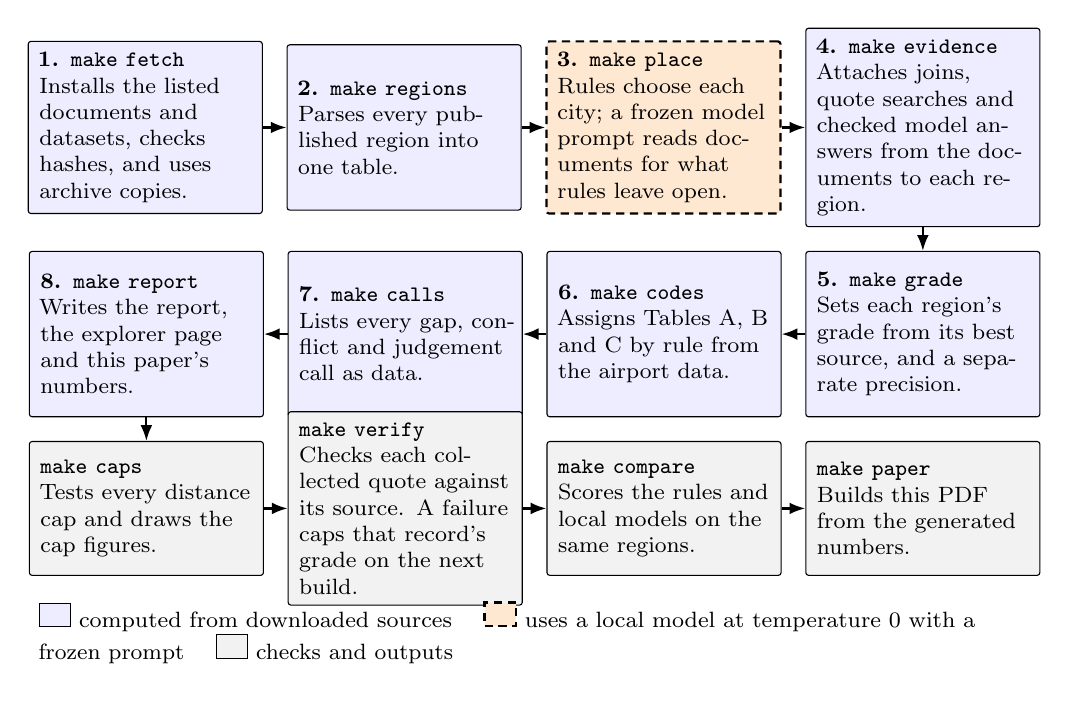
\begin{tikzpicture}[
  node distance=3mm and 3mm, every node/.style={font=\footnotesize},
  box/.style={draw, rounded corners=1pt, text width=0.222\textwidth, align=left, inner sep=4pt, minimum height=21mm, anchor=north west},
  coded/.style={box, fill=blue!7},
  recorded/.style={box, fill=orange!18, densely dashed, thick},
  check/.style={box, fill=black!5, minimum height=17mm},
  flow/.style={-{Latex[length=2mm]}, thick},
]
\node[coded] (fetch) {\textbf{1. \code{make fetch}}\\Installs the listed documents and datasets, checks hashes, and uses archive copies.};
\node[coded, right=of fetch] (regions) {\textbf{2. \code{make regions}}\\Parses every published region into one table.};
\node[recorded, right=of regions] (place) {\textbf{3. \code{make place}}\\Rules choose each city; a frozen model prompt reads documents for what rules leave open.};
\node[coded, right=of place] (evidence) {\textbf{4. \code{make evidence}}\\Attaches joins, quote searches and checked model answers from the documents to each region.};
\node[coded, below=of evidence] (grade) {\textbf{5. \code{make grade}}\\Sets each region's grade from its best source, and a separate precision.};
\node[coded, left=of grade] (codes) {\textbf{6. \code{make codes}}\\Assigns Tables A, B and C by rule from the airport data.};
\node[coded, left=of codes] (calls) {\textbf{7. \code{make calls}}\\Lists every gap, conflict and judgement call as data.};
\node[coded, left=of calls] (report) {\textbf{8. \code{make report}}\\Writes the report, the explorer page and this paper's numbers.};
\draw[flow] (fetch) -- (regions);
\draw[flow] (regions) -- (place);
\draw[flow] (place) -- (evidence);
\draw[flow] (evidence) -- (grade);
\draw[flow] (grade) -- (codes);
\draw[flow] (codes) -- (calls);
\draw[flow] (calls) -- (report);
\node[check, below=of report] (caps) {\textbf{\code{make caps}}\\Tests every distance cap and draws the cap figures.};
\node[check, right=of caps] (verify) {\textbf{\code{make verify}}\\Checks each collected quote against its source. A failure caps that record's grade on the next build.};
\node[check, right=of verify] (compare) {\textbf{\code{make compare}}\\Scores the rules and local models on the same regions.};
\node[check, right=of compare] (paper) {\textbf{\code{make paper}}\\Builds this PDF from the generated numbers.};
\draw[flow] (report) -- (caps);
\draw[flow] (caps) -- (verify);
\draw[flow] (verify) -- (compare);
\draw[flow] (compare) -- (paper);
\node[anchor=north west, below=2mm of caps.south west, anchor=north west, text width=\textwidth, align=left] {%
  \tikz\node[draw, fill=blue!7, minimum width=4mm, minimum height=3mm]{}; computed from downloaded sources \quad
  \tikz\node[draw, fill=orange!18, densely dashed, thick, minimum width=4mm, minimum height=3mm]{}; uses a local model at temperature 0 with a frozen prompt \quad
  \tikz\node[draw, fill=black!5, minimum width=4mm, minimum height=3mm]{}; checks and outputs};
\end{tikzpicture}

\caption{How the data is built. Each box is a command a reader can run. Steps 1 to 8 produce the tables, and the bottom row checks them and builds this paper. Dashed boxes use a local model at temperature 0 with a frozen prompt.}
\label{fig:pipeline}
\end{figure*}

\paragraph{Pipeline.} Figure~\ref{fig:pipeline} shows the steps. A script installs the corpus, parses every vendor list, places regions by rule, reads evidence from the documents, computes codes and writes all outputs, including this paper's numbers and tables. It needs Python with \code{numpy}~\citep{harris2020numpy}, and \code{pdftotext}~\citep{poppler} for PDFs. Tests check behaviour and output invariants: every code exists in its source, codes are unique per vendor, and every region has reasoning and links. A region a vendor adds later is placed by the same rules, and \code{make changes} lists what moved.

\paragraph{Vendors.} We cover \providerCount{} vendors: AWS, Azure, Google Cloud, Alibaba, Oracle, Tencent, Huawei, IBM, OVHcloud, Akamai, Hetzner, Vultr and DigitalOcean. We chose them ourselves, as vendors that sell computing from named regions and publish a region list a script can read. We applied no threshold of revenue or market share, so the set is a sample and not a census, and adding a vendor means adding a parser for its list.

\paragraph{Sources.} Region lists come from the vendors' own pages and APIs, plus botocore for non-commercial AWS partitions~\citep{botocore_endpoints}. We read the region lists and reference datasets on \listsRetrieved{} and last fetched the documents on \documentsRetrieved{}, so every number in this paper describes the lists as they stood then. Our scope is regions open to ordinary customers. The rule is: a region is out of scope when the vendor's own data marks it as sold only to government, classified, financial, self-driving or invited customers. The mark is a botocore partition label for AWS, a region ID pattern for Alibaba and Tencent, and the region name for Huawei. \code{output/excluded\_regions.csv} lists the \excludedCount{} regions this removes, each with its reason and the mark it rests on, and a partition the code has not seen stops the build. The Azure and Oracle lists we read hold commercial regions only; Azure US Government and China and Oracle's government realms are published elsewhere and are not in the corpus. We kept AWS China and the AWS European Sovereign Cloud, which are separate partitions that ordinary businesses can use. Coordinates come from GeoNames~\citep{geonames_readme}. UN/LOCODE comes from a public mirror of the UNECE list~\citep{datasets_unlocode}. Metropolitan codes come from OpenTravelData, an open dataset that is not published by IATA~\citep{opentraveldata}. IATA's official list is a subscription product~\citep{iata_location_database}. CLLI values are six-character city prefixes seen on PeeringDB facilities. They are inferred for an area and were never assigned to a region, as the official registry is proprietary~\citep{iconectiv_ip_faq}.

\paragraph{Corpus.} The input is a fixed list of documents, not a search. \code{sources/documents.csv} holds \corpusDocuments{} documents, \corpusFetched{} of them fetchable, by URL, hash and, where one exists, archive copy, in the manner of LAION's lists of links~\citep{schuhmann2022laion}, and \code{sources/datasets.csv} does the same for datasets. We sourced these documents and built the corpus from them; the choice is ours and is not repeatable. Everything after the list is code or a frozen prompt: a local model reads each document once and says who published it and what kind it is, and that answer sets the source type a grade rests on. A reader's \code{make fetch} downloads each document, prefers an archive copy when a live page no longer matches its hash, installs hand-saved files by hash, and lists what is still missing and where to find it. We list gated documents without storing or quoting them.

\paragraph{Reading evidence from the corpus.} Code reads every record, in three ways. A quote search takes lines that name a region and a place. A retrieval step asks a local model, whose answer code then checks (Section~\ref{sec:llm}). A join reads the facility codes printed under a region's heading in an audit certificate and looks for the same codes in government records that name the operator and a place in the area. A quote counts only if it names the region, names the place outside the region's own names, and is not about a network site such as a Direct Connect location. A place within 100~km of the placed city supports the area, whatever its exact name, because the area is what the tables publish. A checked model answer further away raises a call and moves nothing; a quote-search hit further away is discarded as noise, since documents list many cities. A separate script checks every quote against the cited document, reading PDFs in both text orders, and falls back on that document's saved copy where the live page refuses a script. Of \verifyTotal{} records, \verifyFound{} quotes were found on the live page and \verifySaved{} in a saved copy; \verifyNotFound{} were not found, \verifyUnreachable{} could not be fetched and \verifyNoQuote{} have no quote. A record that fails counts as \code{partial}. A match shows only that the words exist at the source, not that they support the claim, and no person has audited a sample. We publish at city level: a quote holding a street address is cut back to the city.

\paragraph{Testing the quote check.} A quote check only means something if a wrong quote would fail. We broke quotes on purpose, using saved documents, in the manner of mutation testing~\citep{demillo1978hints,jia2011analysis}. Of \mutationControlTotal{} records with a saved document, \mutationControl{} real quotes passed. We then gave each document a quote from a different source: \mutationQuoteFalse{} of \mutationQuoteRecords{} still passed (\mutationQuoteShare{}\%, 95\% interval \mutationQuoteLow{} to \mutationQuoteHigh{}\%). Replacing the city inside the right quote gave \mutationCityFalse{} of \mutationCityRecords{} (\mutationCityShare{}\%, \mutationCityLow{} to \mutationCityHigh{}\%). Length matters here: \mutationShortFalse{} of \mutationShortRecords{} quotes under 20 characters passed wrongly, against \mutationLongFalse{} of \mutationLongRecords{} of 50 characters or more. So short quotes are weak evidence, and the scripted rules ignore them. The test measures whether wrong words get through; it cannot show that right words support a claim.

\section{Results}
\label{sec:results}

\paragraph{Coverage.} Table~\ref{tab:coverage} compares the schemes. Airport codes name every region that has a place, and \placedNone{} has none. Metropolitan codes alone name far fewer, because they exist mainly for cities with several airports, and falling back to airports adds no coverage over airports alone. UN/LOCODE also misses places such as Jerusalem and Zhongwei, and CLLI prefixes mostly cover North America, with some European and a few Asia-Pacific cities.

\begin{table*}[tp]
\centering
\small
\begin{tabular}{lrrr}
\toprule
Scheme & Regions named & Share & Distinct codes \\
\midrule
IATA airport, nearest (nearest airport) & 379 of 380 & 99.7\% & 131 \\
IATA airport, best connected within 200 km (major hub) & 379 of 380 & 99.7\% & 105 \\
IATA airport, major hub within the cap, otherwise nearest (nearby hub) & 379 of 380 & 99.7\% & 125 \\
IATA metro (OpenTravelData) only & 138 of 380 & 36.3\% & 21 \\
IATA metro, airport as fallback & 379 of 380 & 99.7\% & 119 \\
UN/LOCODE & 370 of 380 & 97.4\% & 135 \\
CLLI prefix (inferred) & 138 of 380 & 36.3\% & 33 \\
\bottomrule
\end{tabular}

\caption{How many of the \regionCount{} regions each scheme can name. Coverage depends on the derived places, including low-confidence ones.}
\label{tab:coverage}
\end{table*}

\paragraph{Evidence.} Table~\ref{tab:grades} shows grades by vendor. Hetzner, DigitalOcean, OVHcloud, IBM and Akamai name a place in their lists for every region, and Google Cloud and Oracle for all but one. AWS and Azure account for most regions without one. \gradeVendorDocument{} regions rest on vendor documents, \gradePublicRecord{} on public records, \feedRegions{} on vendor feeds, \gradeReported{} on third-party reporting, \gradePartial{} on partial evidence, \gradeNetwork{} on network presence alone and \gradeAssumed{} on nothing. Precision is coarser than a city for \precisionCoarse{} regions.

\begin{table*}[tp]
\centering
\small
\begin{tabular}{lrrrrrrrr}
\toprule
Vendor & Regions & vendor-stated & vendor-document & public-record & vendor-feed & reported & partial & assumed \\
\midrule
Akamai & 33 & 33 & 0 & 0 & 0 & 0 & 0 & 0 \\
Alibaba & 31 & 28 & 0 & 0 & 0 & 0 & 2 & 1 \\
AWS & 37 & 22 & 2 & 0 & 11 & 1 & 1 & 0 \\
Azure & 59 & 41 & 6 & 5 & 7 & 0 & 0 & 0 \\
DigitalOcean & 16 & 16 & 0 & 0 & 0 & 0 & 0 & 0 \\
Google Cloud & 43 & 42 & 0 & 0 & 1 & 0 & 0 & 0 \\
Hetzner & 6 & 6 & 0 & 0 & 0 & 0 & 0 & 0 \\
Huawei & 28 & 26 & 1 & 0 & 0 & 0 & 1 & 0 \\
IBM & 13 & 13 & 0 & 0 & 0 & 0 & 0 & 0 \\
Oracle & 45 & 44 & 0 & 0 & 0 & 0 & 1 & 0 \\
OVHcloud & 15 & 15 & 0 & 0 & 0 & 0 & 0 & 0 \\
Tencent & 21 & 18 & 1 & 0 & 0 & 0 & 2 & 0 \\
Vultr & 33 & 31 & 1 & 0 & 0 & 0 & 1 & 0 \\
\bottomrule
\end{tabular}

\caption{Strongest evidence grade per region, by vendor.}
\label{tab:grades}
\end{table*}

\paragraph{Audit documents rarely locate regions.} We expected certifications to settle many cases. They mostly did not. AWS's public audit material gives a site count per region and lists cities only for edge and Local Zone sites~\citep{aws_soc3}, and much vendor audit material is gated. Vendor fact sheets name areas, though rarely a region.

\paragraph{Public records.} Government records do not name cloud regions, but some name a vendor's facility codes, and audit certificates tie the same codes to regions. Joining the two gives a route to a place that does not depend on the vendor saying so. \code{make joins} found one for \gradePublicRecord{} Azure regions, from air permits, a federal facility registry, licence filings and a provincial letter, and reports the share of each region's audited codes it joined, from 1 of 10 for \code{centralus} to all 15 for \code{eastus2}. The certificate expired in June 2025~\citep{gsma_microsoft_2024}; we note it, though sites rarely move in a year. The 2024 certificate listed some codes under a different region, so a code list is not fixed, and a code can collide with another operator's, so a join requires the operator's name in the same document. Only Microsoft has such a code list in our corpus.

\paragraph{Vendor IP feeds.} Seven vendors publish IP location feeds, most in the format of RFC~8805~\citep{rfc8805}: AWS, Google Cloud, Microsoft, Akamai, Vultr, DigitalOcean and Hetzner. AWS, Google and Microsoft also publish IP ranges by region, so we take each region's most common city as evidence, and it supports a place only if that city is within 50~km and holds at least half the addresses the feed covers. A feed can support a place but never override one, and it gives metro precision at most. A study of geofeeds found wrong entries for 8.5\% of server addresses and treats feeds as location hints at a 50~km metro level, not as ground truth~\citep{livadariu2024geofeeds}. Our data shows why. Microsoft's file says Dubai for \code{uaecentral}~\citep{azure_geofeed}, which Microsoft lists as Abu Dhabi, and Google's says Taipei for \code{asia-east1}~\citep{gcp_geofeed}, where Google names Changhua County. The strongest evidence for \feedRegions{} regions is a vendor feed, and \feedConflicts{} regions raise a call because the feed disagrees with the place. Microsoft says its file is for geolocation providers, so we cite it and do not redistribute it.

\paragraph{Candidate regions.} The IP ranges of AWS and Google include \candidateCount{} region IDs absent from their published lists. We report them separately and do not count them.

\paragraph{How a place is chosen.} Code applies one order to every region, and the \code{place\_basis} column records which step set the place. The vendor's label or ID comes first (\code{label}). Next comes the vendor's IP feed (\code{feed}), unless a document names another place (\code{document}): a local model read it there, code found its quote, the quote names the region and the document is not a listing or a network page. For a region with no feed the quote need not name the region. A document also sets the place when the label names a town our town list lacks and a vendor sentence locates that town. Then comes the capital when a label names only a country (\code{capital}), and last the place the model recalls with no document (\code{memory}, Section~\ref{sec:llm}). A separate \code{cross\_check} column says whether a second signal agrees or conflicts. \placedByDocument{} regions took their place from a document, \placedByMemory{} from memory alone, and \placedNone{} have no place. No region has a hand-set place.

\paragraph{Vendors label one site several ways.} OVHcloud's regions page lists \code{HIL} as Seattle~\citep{ovh_regions}, while its locations page gives Portland (Hillsboro, Oregon)~\citep{ovh_locations_us}. The same pages give Toronto and Toronto (Cambridge), and Frankfurt and Frankfurt (Limburg). The label comes first, so \code{HIL} is Seattle, and the build raises a call for the other name.

\paragraph{Sources disagree.} Vendors' IP feeds contradict their own lists, as above, and press can differ from both. A disagreement raises a call and leaves the place alone unless a stronger source supports it, in this order: the vendor's list, then a model answer whose quote names the region, then a feed. \code{make area-risk} then sorts weak regions by whether a rival city would change the code, or only the label: \areaRiskSafe{} keep their code against every rival we list, and \areaRiskAtRisk{} could change.

\paragraph{Vendor codes are not always IATA codes.} Oracle's region keys look like airport codes~\citep{oracle_regions}, but \code{LEJ} for Casablanca is Leipzig/Halle, \code{ORF} for Madrid is Norfolk, and \code{HSG} for Batam is Saga in Japan. Vultr's \code{sgp}~\citep{vultr_regions_api} is Shay Gap in Australia~\citep{ourairports_data}, and OVHcloud's \code{LIM} for its Limburg site is Lima's airport code. Importing vendor keys as IATA codes would be wrong.

\paragraph{The tables.} The nearest-airport and major-hub tables disagree on \tableDiffCount{} regions and use \tableADistinct{} and \tableBDistinct{} distinct codes respectively. The nearby-hub table uses \tableCDistinct{} codes, differing from the nearest-airport table on \tableDiffAC{} regions and from the major-hub table on \tableDiffBC{}. Appendix~\ref{app:codes} lists every region in all three. The mechanical rule is repeatable but picks smaller airports: \code{lcy} for London, \code{lga} for New York and \code{mdw} for Chicago, because those airports are closest to the city coordinates. It can also cross a state line: Boydton, Virginia is \code{rdu}, in North Carolina, in the nearest-airport and nearby-hub tables. The major-hub table can reach further: Quincy-Moses Lake, the name Microsoft's feed gives, is \code{eat} by nearest airport and \code{sea} by major hub.

\paragraph{Calls.} The build raised \callCount{} calls, of which \highCallCount{} are high severity (Table~\ref{tab:calls}).

\begin{table}[t]
\centering
\small
\begin{tabular}{llr}
\toprule
Severity & Kind & Count \\
\midrule
high & evidence-conflict & 1 \\
high & gap-iata & 1 \\
high & gap-unmapped & 1 \\
high & vendor-code-conflict & 15 \\
low & city-feed & 19 \\
low & city-reported & 1 \\
low & far-airport & 2 \\
low & nearest-differs-from-hub & 175 \\
low & shared-airport & 57 \\
low & vendor-code-not-iata & 2 \\
medium & candidate-region & 7 \\
medium & city-assumed & 1 \\
medium & city-partial & 8 \\
medium & feed-conflict & 4 \\
medium & gap-unlocode & 10 \\
\bottomrule
\end{tabular}

\caption{Gaps and judgement calls raised by the build.}
\label{tab:calls}
\end{table}

\section{Choosing a distance cap}
\label{sec:cap}

The nearest-airport and major-hub tables are the two ends of one family of rules. A distance cap $c$ blends them: a region keeps its hub if the hub is within $c$ kilometres, and otherwise takes its nearest airport. A cap of zero gives the nearest-airport table and no cap gives the major-hub table. The cap controls a trade-off between overlap across vendors and how accurately a code describes a place. The nearby-hub table uses the cap that a fixed rule selects from the other two, \capUsed{}~km. The rule needs a market radius, which we take from what vendors say a region is.

\paragraph{Where 100~km comes from.} AWS states that all Availability Zones in a region are ``within 100~km (60 miles) of each other''~\citep{aws_regions_az,aws_fault_isolation}, and Microsoft that Azure's zones ``usually are within 100 kilometers of each other''~\citep{azure_availability_zones}. We read these as the largest span vendors publish for one region, so a hub farther than this lies outside what those vendors call one place. We set the market radius $\rho$ to that distance, and use the same 100~km when matching a quote, join or record to a placed city. Only two of our \providerCount{} vendors state such a maximum; Appendix~\ref{app:cap} gives the other vendors' statements and related figures from database engineering.

\paragraph{Rule.} We count pairs of regions from different vendors, and treat regions within $\rho$ kilometres as one market. \emph{Pair recall} is the share of those nearby pairs that have the same code, \emph{false merges} are pairs with the same code that are over $\rho$ apart, and F1 combines the two~\citep{vanrijsbergen1979information}. The result changes only at the distance of a region whose codes differ between the tables, so the script evaluates all \capCount{} candidate caps. Among caps within 0.01 of the best F1, it takes the widest range in which the counts of correct and false pairs do not change, and rounds its midpoint to the nearest 10~km.

\paragraph{Result.} At $\rho=\capRadius$~km the rule selects a cap of \capSelected{}~km: the stable range runs from \capLow{} to \capHigh{}~km, and every cap in it gives the same nearby-hub table (Table~\ref{tab:capnamed}). The vendors' 100~km lies inside that range. Resampling regions or whole cities moves the selected value, so the data fixes a range of equivalent caps, not one value; Appendix~\ref{app:cap} reports the resampling, the sensitivity to $\rho$ and the regions the cap moves off their hub.

\begin{table*}[tp]
\centering
\small
\begin{tabular}{lrrrrrrrr}
\toprule
Cap & Codes & Shared & Recall & FM$>$100 & FM$>$150 & Mean km & Max km & F1 \\
\midrule
0 (nearest airport) & 131 & 310 & 84.4\% & 5 & 0 & 16.0 & 110 & 0.913 \\
50 km & 129 & 315 & 87.1\% & 5 & 0 & 21.2 & 110 & 0.929 \\
84 km (peak) & 125 & 319 & 91.0\% & 5 & 0 & 22.4 & 110 & 0.950 \\
90 km (rule) & 125 & 319 & 91.0\% & 5 & 0 & 22.4 & 110 & 0.950 \\
150 km & 114 & 327 & 91.6\% & 47 & 7 & 27.5 & 150 & 0.932 \\
200 km & 105 & 338 & 91.7\% & 135 & 90 & 35.9 & 193 & 0.891 \\
None (major hub) & 105 & 338 & 91.7\% & 135 & 90 & 35.9 & 193 & 0.891 \\
\bottomrule
\end{tabular}

\caption{Selected caps at $\rho=\capRadius$~km. Codes: distinct codes. Shared: regions on a code used by at least two vendors. FM: false merges over the stated distance in kilometres.}
\label{tab:capnamed}
\end{table*}

\paragraph{What a cap cannot fix.} At the selected cap, \capSplits{} nearby pairs still have different codes. \capBorderSplits{} of them cross a border, such as Singapore with Johor or Batam, Hong Kong with Shenzhen, and Roubaix with Brussels. The same-country rule keeps those apart on purpose. The other \capOtherSplits{} are mostly the Chuncheon pairs. Maximum recall is below 100\% for this reason, and it is a deliberate limit rather than an error.

\section{Placing regions by rule}
\label{sec:placer}

Our reference placements, in \code{evaluation/reference\_placements.csv}, are an earlier placement made outside this pipeline. They feed no table, and we use them only to score methods. The placer uses fixed rules and never reads them. It looks for a city in the vendor's label and region ID, using GeoNames, takes the most common city in the vendor's IP feed where one is tied to the region, and falls back on a country's capital when a label names only a country. It then records two things for each region. The \emph{basis} says what gave the place: \code{label} (the vendor's label or region ID), \code{feed}, \code{capital} or \code{none}; later steps add \code{document} and \code{memory} (Section~\ref{sec:llm}). The \emph{cross-check} says whether a second signal falls within 50~km of the first: \code{agrees}, \code{conflicts}, or blank when there is only one.

The placer gives a place for \placerPlaced{} of \placerRegions{} regions and abstains on \placerAbstained{}. It matches our reference placement within 50~km for \placerAccuracy{}\% of the regions it places (95\% Wilson interval~\citep{wilson1927probable,brown2001interval} \placerAllLow{} to \placerAllHigh{}\%). All \placerAgreedMatched{} of the \placerAgreedRegions{} label placements that a second signal agrees with match. Of the \placerOverturnedTotal{} placements that evidence overturned by hand, it sends \placerOverturnedFlagged{} to review, accepts \placerOverturnedMatching{} at a place matching ours, and accepts \placerOverturnedAccepted{} at the vendor's misleading label. Review means a cross-check that conflicts, or a basis of \code{feed}, \code{capital} or \code{none}. The rules were tuned on these same regions, so this is a description of fit, with no separate test set. Changing the agreement radius, the population limit or the feed share moves the score by a few regions at most (Appendix~\ref{app:methods}).

\section{Placing regions with a local model}
\label{sec:llm}

We then asked whether a language model running on the reader's own machine does better than the rules. All models ran at temperature 0 and a fixed seed, served locally by Docker Model Runner~\citep{docker_model_runner}. We tested three methods with Qwen 3.8~\citep{hf_qwen38}, from the Qwen3 family~\citep{yang2025qwen3}. The \emph{label} method sees only the vendor's region text. The \emph{no documents} method sees only the region ID and name, and answers from what the model remembers. The \emph{RAG} method, retrieval-augmented generation~\citep{lewis2020rag}, cuts each document into passages, embeds them with Qwen's embedding model~\citep{zhang2025qwen3embedding}, keeps only passages that name the region, retrieves the 30 most similar by cosine similarity, as in dense passage retrieval~\citep{karpukhin2020dense}, reranks them with Qwen's reranker~\citep{zhang2025qwen3embedding,nogueira2019passage} and passes the top six to the model. If no passage names the region, the model is not called and the region is left unplaced. Prompts are fixed files in \code{prompts/}, and their hashes are recorded with the results.

Code checks every answer. A quote must appear in the source text and contain the city as a whole word, the city must exist in GeoNames in the stated country, and a state or country given as a city is rejected. Answers that fail are counted, not placed. The no-documents method has no source text, so nothing checks it beyond the GeoNames lookup.

\begin{table*}[tp]
\centering
\small
\begin{tabular}{lrrrrrr}
\toprule
Method & Answers & Matched & 95\% & Review & Overturned & Rules missed \\
\midrule
Rules & 371 of 380 & 365 of 371 & 97--99\% & 38 of 40 & 3 of 5 & 0 \\
Model, label only & 333 of 380 & 329 of 333 & 97--100\% & 4 of 4 & 0 of 0 & 0 \\
Model, no documents & 363 of 380 & 348 of 363 & 93--97\% & 21 of 32 & 3 of 4 & 4 \\
RAG & 321 of 380 & 317 of 321 & 97--100\% & 27 of 29 & 4 of 4 & 5 \\
\bottomrule
\end{tabular}

\caption{Agreement with the reference placements within 50~km. Each match column gives matches out of answers given in that group. The review set is the \llmRulesReviewRegions{} regions the rules send to review, and overturned is the \llmRulesTurnedRegions{} placements changed by hand after reading evidence. The last column counts regions each method matched that the rules did not.}
\label{tab:llm}
\end{table*}

Table~\ref{tab:llm} shows that no model method placed as many regions in agreement as the rules, which answer \llmRulesAnswered{} of \llmRulesRegions{} regions and match \llmRulesMatched{} without a model. Retrieval is the weakest on coverage, answering \llmRagAnswered{}, because for most regions it left unplaced, no text in the vendor's documents named the region. Where it answers it is strong. On the review set, where help is most needed, it matched \llmRagReviewMatched{} of the \llmRagReviewAnswered{} it answered, and it matched \llmRagTurnedMatched{} of the \llmRagTurnedAnswered{} overturned placements it answered, each with a quote. The rules matched \llmRulesTurnedMatched{} of the overturned placements, each from a vendor IP feed.

Retrieval therefore adds to the rules rather than replacing them. It matched \llmRagRescued{} regions the rules did not, each with a quote a reader can check. Its errors include reading a list entry for a US state as the city. A checked quote therefore shows that the words exist in the source, not that the model read them correctly; work on citations from language models separates a quote's presence from its support for the same reason~\citep{gao2023enabling}. Across chat models on the same retrieval, Qwen 3.8 answered \extractRagAnswered{} regions and matched \extractRagMatched{}; Qwen 3.6~\citep{hf_qwen36} \extractRagQwenSixMatched{} of \extractRagQwenSixAnswered{}; and GLM 4.7 Flash~\citep{hf_glm47flash,glm2025glm45} \extractRagGlmMatched{} of \extractRagGlmAnswered{}.

Retrieval needs its filter. Similarity alone retrieves passages that never name the region, so we require retrieved passages to name the region and quotes to name the city.

On regions that two methods both answer, no pair of methods differs after adjustment for multiple tests, so the model methods placed fewer regions, not worse ones. Appendix~\ref{app:methods} gives the paired tests, the agreement between models and the distances of the misses.

\paragraph{What the model adds.} We also compared simpler ways of choosing a city per region from documents. A dictionary-and-rule extractor picked the most common city on lines naming the region: \extractTraditionalMatched{} of \extractTraditionalAnswered{} (\extractTraditionalLow{} to \extractTraditionalHigh{}\%). A statistical version picked the city most over-represented for a region against the vendor's other regions, using smoothed log-odds, a simple form of the measures compared for this task elsewhere~\citep{monroe2008fightin}, which discounts boilerplate: \extractStatisticalMatched{} of \extractStatisticalAnswered{} (\extractStatisticalLow{} to \extractStatisticalHigh{}\%). RAG gave \extractRagMatched{} of \extractRagAnswered{} (\extractRagLow{} to \extractRagHigh{}\%), and a local model reading only the vendor label gave \extractLabelMatched{} of \extractLabelAnswered{} (\extractLabelLow{} to \extractLabelHigh{}\%), which mostly restates labels. For grades, the model changes \modelGainRegions{} regions: \vendorDocWithModel{} reach \code{vendor-document} with its answers and \vendorDocWithoutModel{} without. So most placement needs no model, and recorded answers let a reader rebuild without one.

\section{Comparison with outside sources}
\label{sec:external}

The scores above compare the rules with our own placements. Outside sources give checks we did not make ourselves; none is ground truth. Each comparison was added after the rules it tests were fixed, and those rules have not changed since; later corrections to the choice of UN/LOCODE and to evidence records left the result of every such comparison unchanged.

\paragraph{Codes an operator chose.} Cloudflare names each of its sites with a three-letter code and a city on its public status page~\citep{cloudflare_status}. That is \operatorSites{} choices, made by an operator, of a short code for a known city. We gave our rules each city our town list holds (\operatorSitesResolved{} of them) and counted how often each table gives the code Cloudflare chose. The nearby-hub table agrees on \operatorNearbyHub{} (\operatorNearbyHubShare{}\%), the nearest-airport table on \operatorNearest{} (\operatorNearestShare{}\%) and the major-hub table on \operatorMajorHub{} (\operatorMajorHubShare{}\%). Where they differ, Cloudflare often prefers a city's main international airport to a closer one, as with Bangkok, Buenos Aires and Nairobi, or keeps a code after an airport closed, as with Berlin. These are network sites in city centres, not cloud regions, so the comparison tests naming practice and not where a region is.

\paragraph{Places in another dataset.} The Green Software Foundation's dataset gives a coordinate for AWS, Azure and Google Cloud regions~\citep{gsf_real_time_cloud}. Of the \outsidePlacesCompared{} regions both hold, \outsidePlacesNear{} lie within 50~km of our place (\outsidePlacesShare{}\%, 95\% Wilson interval \outsidePlacesLow{} to \outsidePlacesHigh{}\%), with a median distance of \outsidePlacesMedianKm{}~km. For \outsidePlacesFarStated{} of the \outsidePlacesFar{} that differ, the vendor's own list names our city, such as The Dalles, Council Bluffs or Hamina, and the other dataset gives a point for the wider area or the grid zone. The rest are regions we grade below \code{vendor-stated}, and they are the ones a reader should check first; \code{output/external\_places.csv} lists every distance.

\paragraph{Vendors held out from rule development.} We then fixed the rules and scored them, once, on two vendors that had no part in building them. Each publishes its own sites with a stated city and no login. Both lists were seen when we chose them, so this is a test held out from rule development and not one made unseen. Fastly lists \fastlySites{} sites by city name alone, each with a three-letter code and an approximate coordinate~\citep{fastly_pops}. From the name, the label rule placed \fastlyPlaced{} and abstained on the rest, among them names that several cities share, such as San Jose and Manchester. Of those placed, \fastlyNear{} lie within 50~km of Fastly's own coordinate (\fastlyNearShare{}\%). The misses are mostly namesakes: Naples in Florida was placed in Italy and Santa Clara in California was placed in Cuba. A bare city name is a harder input than a vendor's label, which usually carries a state or country. The code tables agree with Fastly less often than with Cloudflare: the nearby-hub table on \fastlyNearbyHub{} of the \fastlyPlaced{} placed sites (\fastlyNearbyHubShare{}\%), the nearest-airport table on \fastlyNearest{} (\fastlyNearestShare{}\%) and the major-hub table on \fastlyMajorHub{} (\fastlyMajorHubShare{}\%). Fastly's code is an airport in our list for only \fastlyCodeIsAirport{} of those sites, and it often gives several sites in one city different codes. Zenlayer's bare-metal page gives \zenlayerZonesSites{} pairs of a city and a three-letter zone code~\citep{zenlayer_bare_metal}. The rule placed \zenlayerZonesPlaced{} of them, and the nearby-hub table agrees with Zenlayer on \zenlayerZonesNearbyHub{} (\zenlayerZonesNearbyHubShare{}\%), the major-hub table on \zenlayerZonesMajorHub{} (\zenlayerZonesMajorHubShare{}\%) and the nearest-airport table on \zenlayerZonesNearest{} (\zenlayerZonesNearestShare{}\%). Zenlayer's \zenlayerRegions{} compute regions have identifiers such as \code{na-central-2}, printed with the city in brackets~\citep{zenlayer_compute}. The label rule placed \zenlayerRegionsPlaced{} of them. Shown only the identifier and not the city, the local model answered for \zenlayerMemoryAnswered{}, and \zenlayerMemoryNear{} of its answers lie within 50~km of the stated city. The files \code{output/heldout\_*.csv} hold every row. In all three operator lists the nearby-hub table agrees most often.

\section{Threats to validity}
\label{sec:threats}

\paragraph{Agreement is not accuracy.} The scores in Sections~\ref{sec:placer} and~\ref{sec:llm} measure agreement with our reference placements, not truth, and the outside sources of Section~\ref{sec:external} are compiled from vendor statements too. Those placements are ours and draw heavily on the same vendor labels the rules read. The rules, their parameters and the frozen prompts were tuned against them, and we kept no separate test set of regions; Section~\ref{sec:external} scores the fixed rules on two further vendors.

\paragraph{Vendor statements are unverified.} We have no location measurements, so no grade is an independent test of a vendor's claim. Labels and feeds are both the vendor's own statements, so a cross-check that agrees does not mean independently confirmed. The placer cannot find a site that no label, feed or document names.

\paragraph{A label can name a market, not a site.} Four kinds of name are easy to confuse. A \emph{site town} is the town where the buildings stand, as a permit, an audit report or the vendor's own reports give it. A \emph{market name} is the city a vendor sells the region under, usually the nearest large city, and it is what marketing pages and many technical papers use. The \emph{nearest airport} and the \emph{hub} are codes we derive from a place; they name an airport that serves it, not where the region is. Our place is whatever the strongest source names, and a vendor's region list comes first, so where that list gives a market name the place is a market name. We know two such cases, both OVHcloud, and we have not corrected them. The list calls \code{HIL} Seattle, while the vendor's locations page and reports give Hillsboro, Oregon, about 240~km away~\citep{ovh_regions,ovh_locations_us}; its airport codes and UN/LOCODE are therefore Seattle's and not Portland's. The list calls \code{VIN} Washington DC, while the same sources give Vint Hill, Virginia, about 60~km away; the nearby-hub code is Dulles either way, but the nearest-airport code and the UN/LOCODE are Washington's. Other regions graded \code{vendor-stated} may carry a market name that no document in our corpus exposes. A reader who needs the site town should use the evidence records, not the place label.

\paragraph{A quote check shows presence, not support.} A match shows that the words exist at the source, and a model can read the wrong table row: one model placed Google's \code{europe-west4} in Zurich from words that do stand together on the page. To test this, the author opened the source of each of the \reviewRecords{} quoted records, or its archived copy where the live link was dead, and judged whether the page says what the record claims. The author could open \reviewOpened{} of them (\reviewCannotOpen{} failed). In those, the quoted words were on the page in \reviewOnPage{}, and the verdict disagreed with the stance the record carries in \reviewDisagree{}; we withdrew \reviewWithdrawn{} such record from the table afterwards. One person, the author, did this review, so it is not an independent audit.

\paragraph{The corpus was chosen.} We chose the documents, and looked hardest for regions with weak support. A different search would find other documents.

\paragraph{The cap test is partly circular.} The cap and the pair outcome are distances over the same coordinates, so by the triangle inequality a hub within half the radius cannot create a false merge. The market radius, the cap selection rule and the 200~km hub radius are choices we state. Distance is measured to the airport: Chuncheon is about 75~km from Seoul, yet about 120~km from Incheon. The test says nothing about latency.

\paragraph{Places are approximate.} Most places use a city-centre coordinate, while campuses can be far away, and a region can span more than one area: press reports AWS's UAE region in both Abu Dhabi and Dubai~\citep{meed_aws_uae}. Public permits place many cloud buildings in suburbs or nearby towns, and few tie a building to a region. Aragón's orders name AWS's Spanish region and its four towns~\citep{boa_aws_2026a,boa_aws_2026b}, and they agree with Zaragoza. A place the town list lacks falls back on weaker evidence: Google names the port of Eemshaven, and the table gives Groningen from the feed. Oracle's label names Jovanovac, which the list also lacks; its guide locates that region in Kragujevac~\citep{oracle_serbia_realm}, and the rule for such labels places it there.

\paragraph{Models and memory.} The no-documents method cites nothing, a model can state a wrong fact fluently~\citep{ji2023survey}, and its training data may overlap with the vendor labels our placements draw on~\citep{sainz2023nlp}, so its agreement is not independent evidence. Repeated runs gave identical answers on this machine, but settings meant to be deterministic can still vary across runs and hardware~\citep{atil2024nondeterminism}.

\paragraph{Sources drift.} Document access is uneven: one vendor's website refused our client, so its documents were saved by hand and are pinned by hash, and some vendors keep audit reports behind a login, which we did not use. Vendor pages change without notice, as links do across the scholarly web~\citep{klein2014scholarly,jones2016scholarly}, and we cannot redistribute them. A reader without an exact copy gets a run on a different corpus, and possibly different numbers; \code{make fetch} says which files differ, and archive copies restore some.

\section{Discussion}

\paragraph{Which scheme?} For a three-letter resource name, IATA airport codes are the practical choice: they cover the most regions in that length. UN/LOCODE is better for identifying a place, since it covers towns without airports, but it needs five characters. Metropolitan codes group sites usefully yet cannot name most regions on their own. We would not use CLLI as an identifier in open work. We recommend keeping these jobs separate: a stable place identifier in the data, UN/LOCODE as an attribute, and an airport code as the short label.

\paragraph{Regions without a clear city.} A place label is an anchor, not a claim of a site. Where a region has no clear city, or its city rests on weak evidence (\code{vendor-feed} or below), we name it for its metro hub, the airport that serves the market, within the same \capUsed{}~km cap. If the hub is further away, the region takes its nearest airport, and the \code{area\_basis} column records which rule applied. So doubt between towns in one metro does not change the code.

\paragraph{Which table?} For names shared across clouds we suggest the nearby-hub table. It keeps most of the major-hub table's overlap without its long-distance merges, its rule can be stated in one sentence, its limit comes from vendors' own statements, and it agrees most often with the codes each of three operator lists gives its own sites (Section~\ref{sec:external}). We have not tested with users whether any table is easier to work with. The nearest-airport table remains useful where the nearest airport is wanted, and the major-hub table where a single hub name matters more than distance.

\paragraph{Ethics.} The work uses no personal data and involves no human subjects. Every source is a public document. We used no leaked material and no page behind a login, and we list gated documents without storing or quoting them. Where a data centre is can be sensitive, so we publish places at city level only: street addresses, parcel numbers and site coordinates are left out, even where a public filing gives them. Our client identifies itself in every request as \code{OpenCloudModelBot}, with a contact address. \url{https://opencloudmodel.org/crawler} describes it, lists the addresses its requests come from and says how to block it. Before an automated request it reads the site's \code{robots.txt}, and it sends no request that file disallows. Where automated fetching of a document failed, the author opened the page in a browser and saved it.

\paragraph{Reuse terms.} UN/LOCODE is a UN/CEFACT standard, licensed CC BY 4.0~\citep{unece_unlocode_terms}, and we attribute its codes to UNECE. IATA's website terms limit its website content~\citep{iata_terms_of_use}, and we could not read Resolution 763 itself. We found no IATA document that addresses third-party use of location codes, and our airport codes come from OurAirports, not from IATA. We report these statements without drawing legal conclusions, and anyone redistributing these tables should check with the owners.

\paragraph{Next step.} The obvious next step is active measurement, building on constraint-based work~\citep{gondree2013geolocation}: start small instances in each region, measure delay to independent landmarks, and test whether results fit one candidate place. Known-answer controls would come first, using regions whose vendors name a city far from major hubs. Landmark quality matters, since at least 2\% of RIPE Atlas vantage points appear not to be at their reported location~\citep{izhikevich2024rooting}, and close candidates such as Quincy and Seattle may not be separable. A hardware route also exists, in which a host attests a location read from a satellite receiver~\citep{abbas2023enforcing}, but it needs access to the host, so only a provider could deploy it. Results would enter the taxonomy under the reserved \code{measured} grade.

\section{Conclusion}

Most cloud regions can be given a short code, and a majority have a place the vendor names outright. The harder part is being honest about the rest. By publishing evidence, precision and judgement calls with every code, and rebuilding it all from a script, this taxonomy lets a reader see how well each placement is supported, and challenge one region without redoing the table.

\section*{Availability}
The OpenCloudModel Regions code, corpus list and outputs are at \url{https://github.com/opencloudmodelhq/regions}. This paper describes version \datasetVersion{} of the dataset, tagged \code{v\datasetVersion{}} in that repository. That version is archived at \doi{10.5281/zenodo.24215449}. The code is under the Apache License 2.0. The tables, corpus list and other outputs are under CC BY 4.0. This paper is not under that licence; all rights in it are reserved. The outputs draw on GeoNames, OpenTravelData and UN/LOCODE (CC BY 4.0), OurAirports (public domain) and PeeringDB, whose terms still apply to that content, and the reuse terms above apply to the codes. Quotes from vendor and other documents are short quotations; those documents stay under their owners' terms and are not redistributed. The harness downloads them and records their hashes.

\section*{Acknowledgements}
Anthropic's Claude, a large language model, was used for software development, evidence collection and drafting. The author directed this use, checked the results and is responsible for the content. Evidence quotes were checked by a script, as described in Section~\ref{sec:method}, not by a person.

\onecolumn
\bibliographystyle{plainnat}
\bibliography{refs}

\clearpage
\appendix
\section{Distance cap: details}
\label{app:cap}

\paragraph{Limits of that source.} Only two of our \providerCount{} vendors state a maximum, and Microsoft's is hedged by ``usually''. On the pages we read, Google Cloud, Alibaba, Oracle, Tencent and Huawei describe zones only in words such as ``low latency''. IBM and OVHcloud publish minimums instead, at least one mile and at least 30~km in Paris~\citep{ibm_locations,ovh_3az}, and neither bounds a region from above. Some regions are much smaller: IBM describes zones within one campus, and Google says some regions house their zones in one or two data centres~\citep{google_geography}. Some are larger: OVHcloud's SecNumCloud region spans Gravelines, Roubaix and Strasbourg, which by our coordinates lie well over 100~km apart~\citep{ovh_regions}. BSI also uses the same number the other way, as the floor below which two sites should never count as geo-redundant. The figure is a vendor-stated ceiling for zones, which we apply to markets by analogy. It is not a law of networks, since light in fibre covers about 200~km per millisecond, so a 2~ms round trip allows far more than 100~km of path~\citep{singla2014internet}.

\paragraph{Search.} The result changes only at the distance of a region whose codes differ between the tables, so there are \capCount{} candidate caps for the \capRegions{} regions in scope. The script evaluates them all, so no optimiser is needed.

\paragraph{Measures.} We count pairs of regions from different vendors. Fixing a market radius $\rho$ treats regions within $\rho$ kilometres as one market. \emph{Pair recall}, to maximise, is the share of those nearby pairs that have the same code. \emph{False merges}, to minimise, are pairs with the same code that are over $\rho$ apart. F1, their harmonic mean, combines the two~\citep{vanrijsbergen1979information}. We also report regions on a code used by at least two vendors, which is the plain measure of overlap but also rises with false merges, along with distance from a region to its code and the number of distinct codes.

\paragraph{Selection rule.} Code selects the cap. Among caps within 0.01 of the best F1, take the widest range in which the counts of correct and false pairs do not change, then round its midpoint to the nearest 10~km. We prefer this to the raw F1 peak because a peak can rest on a single region.

\paragraph{Result.} At $\rho=\capRadius$~km the rule selects a cap of \capSelected{}~km: the stable range runs from \capLow{} to \capHigh{}~km, with a midpoint of \capMidpoint{}~km. The nearby-hub table uses this cap. The vendors' 100~km also lies inside the range, where the pair counts do not change, so it would give the same codes. The rule is not steady, however. Across \capRuleRuns{} resamples of the regions it chose \capSelected{}~km \capRuleShare{}\% of the time, with a median of \capRuleMedian{}~km and a 5th to 95th percentile range of \capRuleLow{} to \capRuleHigh{}~km. Dropping one vendor at a time keeps \capSelected{}~km for \capRuleKept{} of \capRuleVendors{} vendors and moves it for the others: \capRuleMoved{}. Regions in one city are not independent, so we also resampled whole cities, as in a cluster bootstrap~\citep{field2007bootstrapping}. That is less steady still: \capCityShare{}\% at \capSelected{}~km, with a median of \capCityMedian{}~km and a range of \capCityLow{} to \capCityHigh{}~km. So the data fixes a range of equivalent caps rather than one value, and any cap in it gives the same nearby-hub table.

\paragraph{A merge interval.} A single cap is not well determined, so we also report an interval: caps that add no false merge and keep at least 99\% of the correct pairs reachable without one. At $\rho=\capRadius$~km it runs from \capIntervalLow{}~km up to, but not including, \capIntervalHigh{}~km, the cap at which the first new false merge appears. Every cap in it gives \capIntervalPairs{} correct pairs and \capIntervalFalse{} false merges, all of them already in the nearest-airport table. Here it is the same as the stable range, and it holds the selected \capSelected{}~km. Resampling cities moves both edges. The upper edge has a median of \capCityUpperMedian{}~km (5th to 95th percentile \capCityUpperLow{} to \capCityUpperHigh{}~km), so it rarely falls below the full-data value. The lower edge moves far more, with a median of \capCityLowerMedian{}~km and a range of \capCityLowerLow{} to \capCityLowerHigh{}~km. The interval contains \capSelected{}~km in \capRegionHolds{}\% of region resamples and \capCityHolds{}\% of city resamples. The 99\% is our choice. Figure~\ref{fig:capbands} shows why overlap stops being useful. The new pairs are all correct until the \capMixedLow{} to \capMixedHigh{}~km band, which contains both Chuncheon joining Seoul (\capMixedGood{} correct pairs) and G\"avle joining Stockholm (\capMixedBad{} false pairs). Every later pair is a false merge.

\paragraph{The raw peak.} F1 is highest at \capPeak{}~km, the start of the stable range, so that value and \capUsed{}~km give the same pairs. Dropping one vendor mostly leaves the peak there (Table~\ref{tab:capstability}). In a bootstrap of the regions~\citep{efron1979bootstrap}, the 5th to 95th percentile of the best cap runs from \capBootLow{} to \capBootHigh{}~km. A cap above the range would gain \capMixedGood{} Chuncheon pairs at the cost of \capMixedBad{} G\"avle pairs. A named exception could restore the first without the second.

\paragraph{Sensitivity to the radius.} The answer depends on $\rho$ (Figure~\ref{fig:capf1}, Table~\ref{tab:capradius}), and the data cannot choose $\rho$, because a larger market radius simply tolerates larger merges. The rule selects the same cap at 75 and 100~km but very different ones at 50 and 150~km. In OpenTravelData~\citep{opentraveldata}, an unofficial source, 95\% of \metroLinks{} links between an airport and its metropolitan code are within \metroNinetyFive{}~km and 99\% are within \metroNinetyNine{}~km, so airline practice brackets the figure without pointing to it.

\begin{figure}[htbp]
\centering
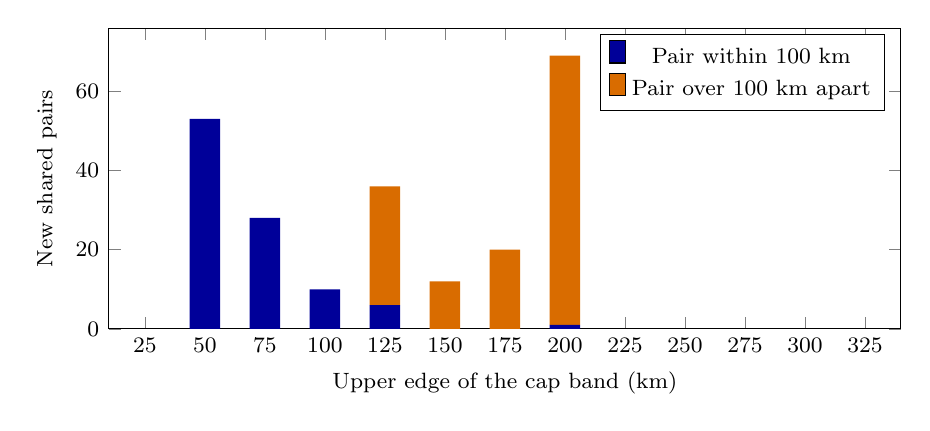
\begin{tikzpicture}
\begin{axis}[ybar stacked,bar width=11pt,width=0.96\linewidth,height=5.4cm,ymin=0,xmin=10,xmax=340,xtick=data,xlabel={Upper edge of the cap band (km)},ylabel={New shared pairs},legend style={font=\footnotesize},tick label style={font=\footnotesize},label style={font=\footnotesize},title style={font=\footnotesize\bfseries}]
\addplot[fill=blue!60!black,draw=none] coordinates {(25.00,0.0000) (50.00,53.0000) (75.00,28.0000) (100.00,10.0000) (125.00,6.0000) (150.00,0.0000) (175.00,0.0000) (200.00,1.0000) (225.00,0.0000) (250.00,0.0000) (275.00,0.0000) (300.00,0.0000) (325.00,0.0000)};
\addplot[fill=orange!85!black,draw=none] coordinates {(25.00,0.0000) (50.00,0.0000) (75.00,0.0000) (100.00,0.0000) (125.00,30.0000) (150.00,12.0000) (175.00,20.0000) (200.00,68.0000) (225.00,0.0000) (250.00,0.0000) (275.00,0.0000) (300.00,0.0000) (325.00,0.0000)};
\legend{Pair within 100 km,Pair over 100 km apart}
\end{axis}
\end{tikzpicture}

\caption{New cross-vendor pairs that come to share a code as the cap rises, in 25~km bands, at $\rho=\capRadius$~km.}
\label{fig:capbands}
\end{figure}

\begin{figure}[htbp]
\centering
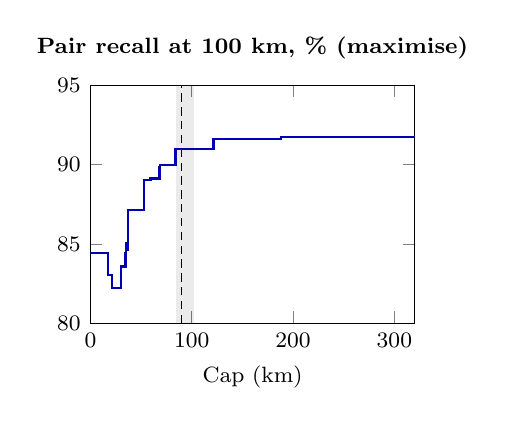
\begin{tikzpicture}
\begin{axis}[width=0.47\linewidth,height=4.6cm,xmin=0,xmax=320,ymin=80,ymax=95,title={Pair recall at 100 km, \% (maximise)},xlabel={Cap (km)},tick label style={font=\footnotesize},label style={font=\footnotesize},title style={font=\footnotesize\bfseries}]
\fill[black,opacity=0.08] (axis cs:84.06,80) rectangle (axis cs:102.47,95);
\draw[black,densely dashed] (axis cs:90,80) -- (axis cs:90,95);
\addplot[const plot mark left,thick,blue!70!black,no markers] coordinates {(0.00,84.4142) (12.80,84.4142) (17.36,83.0544) (17.67,83.0544) (19.38,83.0544) (19.45,83.0544) (19.91,83.0544) (20.85,83.0544) (21.31,82.2176) (22.89,82.2176) (23.13,82.2176) (23.51,82.2176) (25.04,82.2176) (25.47,82.2176) (28.92,82.2176) (29.68,82.2176) (30.15,83.5774) (31.07,83.5774) (34.15,83.5774) (34.27,83.5774) (34.69,84.4142) (34.82,85.0418) (34.95,84.6234) (36.35,84.6234) (36.70,87.1339) (40.41,87.1339) (44.07,87.1339) (47.75,87.1339) (52.59,89.0167) (59.32,89.1213) (68.26,89.8536) (68.84,89.9582) (84.06,91.0042) (101.37,91.0042) (102.47,91.0042) (110.59,91.0042) (111.08,91.0042) (117.62,91.0042) (121.52,91.6318) (121.69,91.6318) (122.12,91.6318) (122.76,91.6318) (125.71,91.6318) (131.64,91.6318) (132.45,91.6318) (139.11,91.6318) (142.83,91.6318) (142.86,91.6318) (146.10,91.6318) (149.97,91.6318) (154.64,91.6318) (157.99,91.6318) (165.66,91.6318) (165.79,91.6318) (170.37,91.6318) (176.07,91.6318) (178.09,91.6318) (183.33,91.6318) (186.70,91.6318) (188.07,91.6318) (188.38,91.7364) (191.88,91.7364) (192.60,91.7364) (193.28,91.7364) (320.00,91.7364)};
\end{axis}
\end{tikzpicture}\hfill
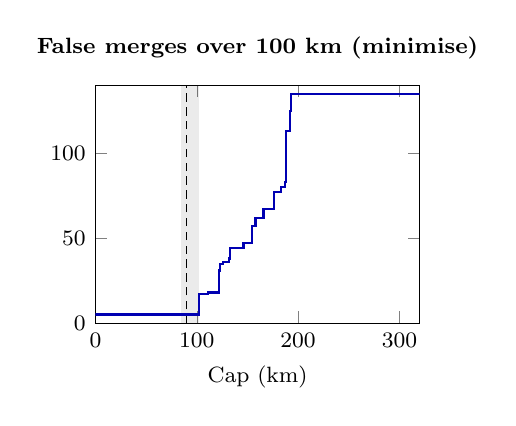
\begin{tikzpicture}
\begin{axis}[width=0.47\linewidth,height=4.6cm,xmin=0,xmax=320,ymin=0,ymax=140,title={False merges over 100 km (minimise)},xlabel={Cap (km)},tick label style={font=\footnotesize},label style={font=\footnotesize},title style={font=\footnotesize\bfseries}]
\fill[black,opacity=0.08] (axis cs:84.06,0) rectangle (axis cs:102.47,140);
\draw[black,densely dashed] (axis cs:90,0) -- (axis cs:90,140);
\addplot[const plot mark left,thick,blue!70!black,no markers] coordinates {(0.00,5.0000) (12.80,5.0000) (17.36,5.0000) (17.67,5.0000) (19.38,5.0000) (19.45,5.0000) (19.91,5.0000) (20.85,5.0000) (21.31,5.0000) (22.89,5.0000) (23.13,5.0000) (23.51,5.0000) (25.04,5.0000) (25.47,5.0000) (28.92,5.0000) (29.68,5.0000) (30.15,5.0000) (31.07,5.0000) (34.15,5.0000) (34.27,5.0000) (34.69,5.0000) (34.82,5.0000) (34.95,5.0000) (36.35,5.0000) (36.70,5.0000) (40.41,5.0000) (44.07,5.0000) (47.75,5.0000) (52.59,5.0000) (59.32,5.0000) (68.26,5.0000) (68.84,5.0000) (84.06,5.0000) (101.37,5.0000) (102.47,17.0000) (110.59,17.0000) (111.08,18.0000) (117.62,18.0000) (121.52,18.0000) (121.69,26.0000) (122.12,31.0000) (122.76,35.0000) (125.71,36.0000) (131.64,38.0000) (132.45,44.0000) (139.11,44.0000) (142.83,44.0000) (142.86,44.0000) (146.10,47.0000) (149.97,47.0000) (154.64,57.0000) (157.99,62.0000) (165.66,62.0000) (165.79,67.0000) (170.37,67.0000) (176.07,77.0000) (178.09,77.0000) (183.33,80.0000) (186.70,83.0000) (188.07,103.0000) (188.38,113.0000) (191.88,125.0000) (192.60,134.0000) (193.28,135.0000) (320.00,135.0000)};
\end{axis}
\end{tikzpicture}

\medskip
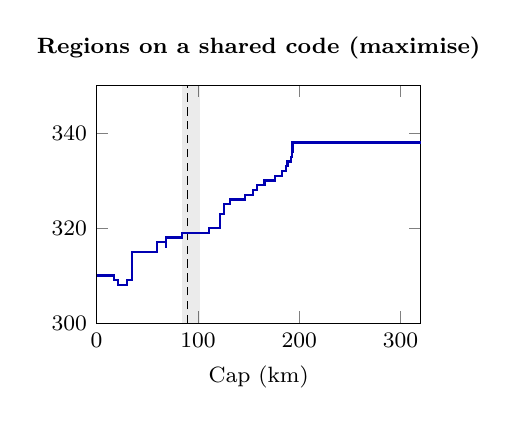
\begin{tikzpicture}
\begin{axis}[width=0.47\linewidth,height=4.6cm,xmin=0,xmax=320,ymin=300,ymax=350,title={Regions on a shared code (maximise)},xlabel={Cap (km)},tick label style={font=\footnotesize},label style={font=\footnotesize},title style={font=\footnotesize\bfseries}]
\fill[black,opacity=0.08] (axis cs:84.06,300) rectangle (axis cs:102.47,350);
\draw[black,densely dashed] (axis cs:90,300) -- (axis cs:90,350);
\addplot[const plot mark left,thick,blue!70!black,no markers] coordinates {(0.00,310.0000) (12.80,310.0000) (17.36,309.0000) (17.67,309.0000) (19.38,309.0000) (19.45,309.0000) (19.91,309.0000) (20.85,309.0000) (21.31,308.0000) (22.89,308.0000) (23.13,308.0000) (23.51,308.0000) (25.04,308.0000) (25.47,308.0000) (28.92,308.0000) (29.68,308.0000) (30.15,309.0000) (31.07,309.0000) (34.15,309.0000) (34.27,309.0000) (34.69,310.0000) (34.82,313.0000) (34.95,315.0000) (36.35,315.0000) (36.70,315.0000) (40.41,315.0000) (44.07,315.0000) (47.75,315.0000) (52.59,315.0000) (59.32,317.0000) (68.26,316.0000) (68.84,318.0000) (84.06,319.0000) (101.37,319.0000) (102.47,319.0000) (110.59,319.0000) (111.08,320.0000) (117.62,320.0000) (121.52,321.0000) (121.69,322.0000) (122.12,323.0000) (122.76,323.0000) (125.71,325.0000) (131.64,326.0000) (132.45,326.0000) (139.11,326.0000) (142.83,326.0000) (142.86,326.0000) (146.10,327.0000) (149.97,327.0000) (154.64,328.0000) (157.99,329.0000) (165.66,329.0000) (165.79,330.0000) (170.37,330.0000) (176.07,331.0000) (178.09,331.0000) (183.33,332.0000) (186.70,333.0000) (188.07,333.0000) (188.38,334.0000) (191.88,335.0000) (192.60,336.0000) (193.28,338.0000) (320.00,338.0000)};
\end{axis}
\end{tikzpicture}\hfill
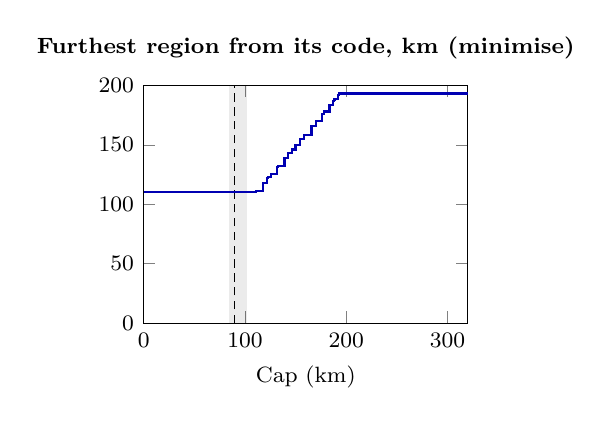
\begin{tikzpicture}
\begin{axis}[width=0.47\linewidth,height=4.6cm,xmin=0,xmax=320,ymin=0,ymax=200,title={Furthest region from its code, km (minimise)},xlabel={Cap (km)},tick label style={font=\footnotesize},label style={font=\footnotesize},title style={font=\footnotesize\bfseries}]
\fill[black,opacity=0.08] (axis cs:84.06,0) rectangle (axis cs:102.47,200);
\draw[black,densely dashed] (axis cs:90,0) -- (axis cs:90,200);
\addplot[const plot mark left,thick,blue!70!black,no markers] coordinates {(0.00,110.4387) (12.80,110.4387) (17.36,110.4387) (17.67,110.4387) (19.38,110.4387) (19.45,110.4387) (19.91,110.4387) (20.85,110.4387) (21.31,110.4387) (22.89,110.4387) (23.13,110.4387) (23.51,110.4387) (25.04,110.4387) (25.47,110.4387) (28.92,110.4387) (29.68,110.4387) (30.15,110.4387) (31.07,110.4387) (34.15,110.4387) (34.27,110.4387) (34.69,110.4387) (34.82,110.4387) (34.95,110.4387) (36.35,110.4387) (36.70,110.4387) (40.41,110.4387) (44.07,110.4387) (47.75,110.4387) (52.59,110.4387) (59.32,110.4387) (68.26,110.4387) (68.84,110.4387) (84.06,110.4387) (101.37,110.4387) (102.47,110.4387) (110.59,110.5943) (111.08,111.0803) (117.62,117.6153) (121.52,121.5183) (121.69,121.6887) (122.12,122.1152) (122.76,122.7610) (125.71,125.7067) (131.64,131.6389) (132.45,132.4543) (139.11,139.1144) (142.83,142.8344) (142.86,142.8619) (146.10,146.0988) (149.97,149.9715) (154.64,154.6437) (157.99,157.9948) (165.66,165.6552) (165.79,165.7942) (170.37,170.3664) (176.07,176.0716) (178.09,178.0854) (183.33,183.3345) (186.70,186.6972) (188.07,188.0684) (188.38,188.3797) (191.88,191.8822) (192.60,192.5966) (193.28,193.2778) (320.00,193.2778)};
\end{axis}
\end{tikzpicture}

\caption{Four measures across all candidate caps. The shaded range is where pair counts do not change, and the dashed line is the selected cap.}
\label{fig:capmeasures}
\end{figure}

\begin{figure}[htbp]
\centering
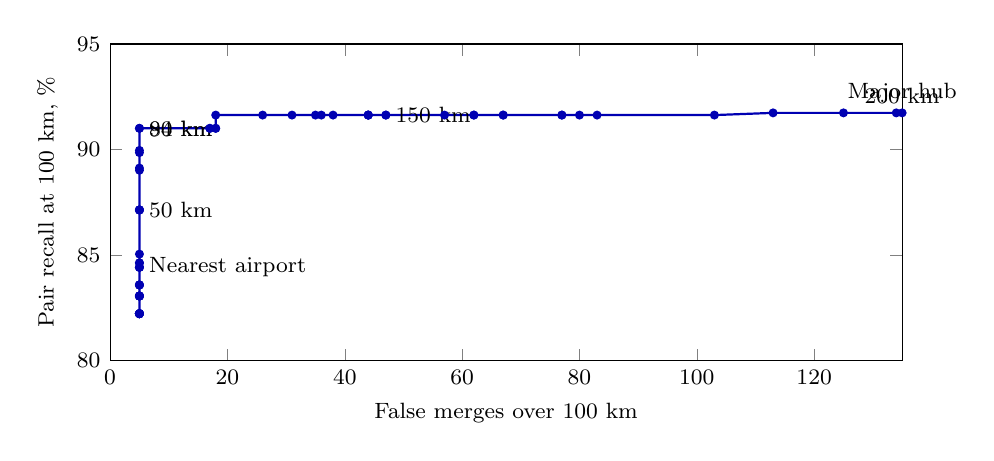
\begin{tikzpicture}
\begin{axis}[width=0.96\linewidth,height=5.6cm,xmin=0,xmax=135,ymin=80,ymax=95,clip=false,xlabel={False merges over 100 km},ylabel={Pair recall at 100 km, \%},tick label style={font=\footnotesize},label style={font=\footnotesize},title style={font=\footnotesize\bfseries}]
\addplot[thick,blue!70!black,mark=*,mark size=1.2pt] coordinates {(5.00,84.4142) (5.00,84.4142) (5.00,83.0544) (5.00,83.0544) (5.00,83.0544) (5.00,83.0544) (5.00,83.0544) (5.00,83.0544) (5.00,82.2176) (5.00,82.2176) (5.00,82.2176) (5.00,82.2176) (5.00,82.2176) (5.00,82.2176) (5.00,82.2176) (5.00,82.2176) (5.00,83.5774) (5.00,83.5774) (5.00,83.5774) (5.00,83.5774) (5.00,84.4142) (5.00,85.0418) (5.00,84.6234) (5.00,84.6234) (5.00,87.1339) (5.00,87.1339) (5.00,87.1339) (5.00,87.1339) (5.00,89.0167) (5.00,89.1213) (5.00,89.8536) (5.00,89.9582) (5.00,91.0042) (5.00,91.0042) (17.00,91.0042) (17.00,91.0042) (18.00,91.0042) (18.00,91.0042) (18.00,91.6318) (26.00,91.6318) (31.00,91.6318) (35.00,91.6318) (36.00,91.6318) (38.00,91.6318) (44.00,91.6318) (44.00,91.6318) (44.00,91.6318) (44.00,91.6318) (47.00,91.6318) (47.00,91.6318) (57.00,91.6318) (62.00,91.6318) (62.00,91.6318) (67.00,91.6318) (67.00,91.6318) (77.00,91.6318) (77.00,91.6318) (80.00,91.6318) (83.00,91.6318) (103.00,91.6318) (113.00,91.7364) (125.00,91.7364) (134.00,91.7364) (135.00,91.7364)};
\node[font=\footnotesize,anchor=west] at (axis cs:5,84.41) {Nearest airport};
\node[font=\footnotesize,anchor=west] at (axis cs:5,87.13) {50 km};
\node[font=\footnotesize,anchor=west] at (axis cs:5,91.00) {84 km};
\node[font=\footnotesize,anchor=west] at (axis cs:5,91.00) {90 km};
\node[font=\footnotesize,anchor=west] at (axis cs:47,91.63) {150 km};
\node[font=\footnotesize,anchor=south] at (axis cs:135,91.74) {200 km};
\node[font=\footnotesize,anchor=south] at (axis cs:135,91.74) {Major hub};
\end{axis}
\end{tikzpicture}

\caption{Recall against false merges, with one point for each candidate cap. Beyond the F1 peak, recall does not rise and false merges do.}
\label{fig:captradeoff}
\end{figure}

\begin{figure}[htbp]
\centering
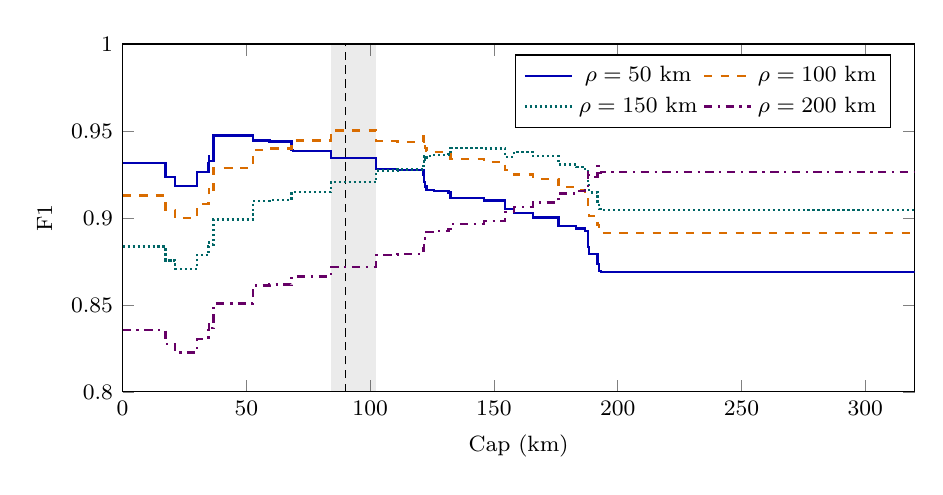
\begin{tikzpicture}
\begin{axis}[width=0.96\linewidth,height=6cm,xmin=0,xmax=320,ymin=0.8,ymax=1,xlabel={Cap (km)},ylabel={F1},legend pos=north east,legend columns=2,legend style={font=\footnotesize},tick label style={font=\footnotesize},label style={font=\footnotesize},title style={font=\footnotesize\bfseries}]
\fill[black,opacity=0.08] (axis cs:84.06,0.8) rectangle (axis cs:102.47,1);
\draw[black,densely dashed] (axis cs:90,0.8) -- (axis cs:90,1);
\addplot[const plot mark left,thick,no markers,blue!70!black,solid] coordinates {(0.00,0.9316) (12.80,0.9316) (17.36,0.9234) (17.67,0.9234) (19.38,0.9234) (19.45,0.9234) (19.91,0.9234) (20.85,0.9234) (21.31,0.9184) (22.89,0.9184) (23.13,0.9184) (23.51,0.9184) (25.04,0.9184) (25.47,0.9184) (28.92,0.9184) (29.68,0.9184) (30.15,0.9266) (31.07,0.9266) (34.15,0.9266) (34.27,0.9266) (34.69,0.9316) (34.82,0.9353) (34.95,0.9328) (36.35,0.9328) (36.70,0.9474) (40.41,0.9474) (44.07,0.9474) (47.75,0.9474) (52.59,0.9446) (59.32,0.9440) (68.26,0.9392) (68.84,0.9387) (84.06,0.9345) (101.37,0.9345) (102.47,0.9283) (110.59,0.9283) (111.08,0.9278) (117.62,0.9278) (121.52,0.9247) (121.69,0.9206) (122.12,0.9181) (122.76,0.9161) (125.71,0.9156) (131.64,0.9146) (132.45,0.9116) (139.11,0.9116) (142.83,0.9116) (142.86,0.9116) (146.10,0.9101) (149.97,0.9101) (154.64,0.9051) (157.99,0.9027) (165.66,0.9027) (165.79,0.9003) (170.37,0.9003) (176.07,0.8954) (178.09,0.8954) (183.33,0.8940) (186.70,0.8926) (188.07,0.8831) (188.38,0.8791) (191.88,0.8736) (192.60,0.8695) (193.28,0.8690) (320.00,0.8690)};
\addplot[const plot mark left,thick,no markers,orange!85!black,dashed] coordinates {(0.00,0.9129) (12.80,0.9129) (17.36,0.9048) (17.67,0.9048) (19.38,0.9048) (19.45,0.9048) (19.91,0.9048) (20.85,0.9048) (21.31,0.8998) (22.89,0.8998) (23.13,0.8998) (23.51,0.8998) (25.04,0.8998) (25.47,0.8998) (28.92,0.8998) (29.68,0.8998) (30.15,0.9080) (31.07,0.9080) (34.15,0.9080) (34.27,0.9080) (34.69,0.9129) (34.82,0.9166) (34.95,0.9141) (36.35,0.9141) (36.70,0.9287) (40.41,0.9287) (44.07,0.9287) (47.75,0.9287) (52.59,0.9393) (59.32,0.9399) (68.26,0.9440) (68.84,0.9445) (84.06,0.9503) (101.37,0.9503) (102.47,0.9441) (110.59,0.9441) (111.08,0.9436) (117.62,0.9436) (121.52,0.9470) (121.69,0.9429) (122.12,0.9404) (122.76,0.9384) (125.71,0.9379) (131.64,0.9369) (132.45,0.9339) (139.11,0.9339) (142.83,0.9339) (142.86,0.9339) (146.10,0.9324) (149.97,0.9324) (154.64,0.9275) (157.99,0.9250) (165.66,0.9250) (165.79,0.9226) (170.37,0.9226) (176.07,0.9178) (178.09,0.9178) (183.33,0.9163) (186.70,0.9149) (188.07,0.9054) (188.38,0.9013) (191.88,0.8958) (192.60,0.8917) (193.28,0.8913) (320.00,0.8913)};
\addplot[const plot mark left,thick,no markers,teal!80!black,densely dotted] coordinates {(0.00,0.8836) (12.80,0.8836) (17.36,0.8756) (17.67,0.8756) (19.38,0.8756) (19.45,0.8756) (19.91,0.8756) (20.85,0.8756) (21.31,0.8707) (22.89,0.8707) (23.13,0.8707) (23.51,0.8707) (25.04,0.8707) (25.47,0.8707) (28.92,0.8707) (29.68,0.8707) (30.15,0.8787) (31.07,0.8787) (34.15,0.8787) (34.27,0.8787) (34.69,0.8836) (34.82,0.8872) (34.95,0.8848) (36.35,0.8848) (36.70,0.8991) (40.41,0.8991) (44.07,0.8991) (47.75,0.8991) (52.59,0.9097) (59.32,0.9102) (68.26,0.9143) (68.84,0.9149) (84.06,0.9206) (101.37,0.9206) (102.47,0.9273) (110.59,0.9273) (111.08,0.9279) (117.62,0.9279) (121.52,0.9313) (121.69,0.9357) (122.12,0.9333) (122.76,0.9355) (125.71,0.9360) (131.64,0.9371) (132.45,0.9404) (139.11,0.9404) (142.83,0.9404) (142.86,0.9404) (146.10,0.9400) (149.97,0.9400) (154.64,0.9352) (157.99,0.9379) (165.66,0.9379) (165.79,0.9355) (170.37,0.9355) (176.07,0.9308) (178.09,0.9308) (183.33,0.9294) (186.70,0.9280) (188.07,0.9187) (188.38,0.9147) (191.88,0.9093) (192.60,0.9053) (193.28,0.9048) (320.00,0.9048)};
\addplot[const plot mark left,thick,no markers,violet!80!black,dashdotted] coordinates {(0.00,0.8354) (12.80,0.8354) (17.36,0.8276) (17.67,0.8276) (19.38,0.8276) (19.45,0.8276) (19.91,0.8276) (20.85,0.8276) (21.31,0.8227) (22.89,0.8227) (23.13,0.8227) (23.51,0.8227) (25.04,0.8227) (25.47,0.8227) (28.92,0.8227) (29.68,0.8227) (30.15,0.8306) (31.07,0.8306) (34.15,0.8306) (34.27,0.8306) (34.69,0.8354) (34.82,0.8390) (34.95,0.8366) (36.35,0.8366) (36.70,0.8508) (40.41,0.8508) (44.07,0.8508) (47.75,0.8508) (52.59,0.8612) (59.32,0.8617) (68.26,0.8657) (68.84,0.8663) (84.06,0.8719) (101.37,0.8719) (102.47,0.8787) (110.59,0.8787) (111.08,0.8792) (117.62,0.8792) (121.52,0.8825) (121.69,0.8869) (122.12,0.8897) (122.76,0.8918) (125.71,0.8924) (131.64,0.8935) (132.45,0.8967) (139.11,0.8967) (142.83,0.8967) (142.86,0.8967) (146.10,0.8983) (149.97,0.8983) (154.64,0.9036) (157.99,0.9063) (165.66,0.9063) (165.79,0.9089) (170.37,0.9089) (176.07,0.9141) (178.09,0.9141) (183.33,0.9157) (186.70,0.9173) (188.07,0.9275) (188.38,0.9237) (191.88,0.9297) (192.60,0.9258) (193.28,0.9263) (320.00,0.9263)};
\legend{$\rho=50$ km,$\rho=100$ km,$\rho=150$ km,$\rho=200$ km}
\end{axis}
\end{tikzpicture}

\caption{F1 by cap for four market radii. The shaded range and dashed line are those for $\rho=\capRadius$~km.}
\label{fig:capf1}
\end{figure}

\begin{table}[htbp]
\centering
\small
\begin{tabular}{lrrr}
\toprule
Market radius $\rho$ & F1 peak & Bootstrap 5--95\% & Rule selects \\
\midrule
50 km & 37 km & 35 to 53 km & 40 km \\
75 km & 69 km & 53 to 122 km & 90 km \\
100 km & 84 km & 59 to 122 km & 90 km \\
150 km & 132 km & 122 to 158 km & 140 km \\
200 km & 192 km & 188 to 193 km & 190 km \\
\bottomrule
\end{tabular}

\caption{Results by market radius.}
\label{tab:capradius}
\end{table}

\begin{table}[htbp]
\centering
\small
\begin{tabular}{lrr}
\toprule
Test & Regions & F1 peak \\
\midrule
All regions & 379 & 84 km \\
City-level locations only & 335 & 69 km \\
Without Akamai & 346 & 84 km \\
Without Alibaba & 349 & 84 km \\
Without AWS & 342 & 84 km \\
Without Azure & 320 & 68 km \\
Without DigitalOcean & 363 & 84 km \\
Without Google Cloud & 336 & 84 km \\
Without Hetzner & 373 & 84 km \\
Without Huawei & 351 & 84 km \\
Without IBM & 366 & 84 km \\
Without Oracle & 334 & 84 km \\
Without OVHcloud & 364 & 84 km \\
Without Tencent & 358 & 84 km \\
Without Vultr & 346 & 84 km \\
\bottomrule
\end{tabular}

\caption{F1 peak at $\rho=\capRadius$~km on subsets.}
\label{tab:capstability}
\end{table}

\begin{table}[htbp]
\centering
\small
\begin{tabular}{lllrrrr}
\toprule
Vendor & Region & Place & Hub & km & Instead & km \\
\midrule
Alibaba & cn-hangzhou & Hangzhou & PVG & 183 & HGH & 26 \\
Alibaba & cn-heyuan & Heyuan & CAN & 146 & HUZ & 76 \\
Alibaba & cn-shenzhen & Shenzhen & CAN & 123 & SZX & 29 \\
Alibaba & cn-wulanchabu & Ulanqab & HET & 111 & UCB & 15 \\
Alibaba & cn-zhangjiakou & Zhangjiakou & PEK & 166 & ZQZ & 7 \\
Alibaba & cn-zhongwei & Zhongwei & LHW & 178 & ZHY & 8 \\
AWS & cn-northwest-1 & Zhongwei & LHW & 178 & ZHY & 8 \\
AWS & eu-south-2 & Zaragoza & PNA & 139 & ZAZ & 14 \\
AWS & mx-central-1 & Queretaro & MEX & 188 & QRO & 21 \\
Azure & centralindia & Pune & BOM & 122 & PNQ & 10 \\
Azure & centralus & Des Moines & OMA & 193 & DSM & 8 \\
Azure & mexicocentral & Queretaro & MEX & 188 & QRO & 21 \\
Azure & norwaywest & Stavanger & BGO & 150 & SVG & 12 \\
Azure & southcentralus & San Antonio & AUS & 118 & SAT & 12 \\
Azure & swedencentral & Gävle & ARN & 122 & BLE & 93 \\
Azure & uaecentral & Abu Dhabi & DXB & 132 & AUH & 26 \\
Azure & ukwest & Cardiff & LHR & 188 & CWL & 15 \\
Azure & westcentralus & Cheyenne & DEN & 143 & CYS & 2 \\
Azure & westus2 & Quincy-Moses Lake & SEA & 187 & EAT & 32 \\
DigitalOcean & ric1 & Richmond & IAD & 155 & RIC & 14 \\
Google Cloud & asia-east1 & Changhua & TPE & 132 & RMQ & 23 \\
Google Cloud & europe-north1 & Hamina & HEL & 126 & LPP & 74 \\
Google Cloud & europe-west12 & Turin & MXP & 102 & TRN & 15 \\
Google Cloud & europe-west4 & Groningen & AMS & 158 & GRQ & 11 \\
Google Cloud & northamerica-south1 & Queretaro & MEX & 188 & QRO & 21 \\
Hetzner & fsn1 & Falkenstein & NUE & 143 & LEJ & 105 \\
Hetzner & nbg1 & Nuremberg & FRA & 192 & NUE & 5 \\
Huawei & cn-north-12 & Shijiazhuang & TYN & 166 & SJW & 33 \\
Huawei & cn-north-9 & Ulanqab & HET & 111 & UCB & 15 \\
Huawei & cn-south-2 & Shenzhen & CAN & 123 & SZX & 29 \\
Oracle & ap-chuncheon-1 & Chuncheon & ICN & 122 & WJU & 54 \\
Oracle & eu-jovanovac-1 & Kragujevac & BEG & 101 & KVO & 34 \\
Oracle & eu-turin-1 & Turin & MXP & 102 & TRN & 15 \\
Oracle & me-abudhabi-1 & Abu Dhabi & DXB & 132 & AUH & 26 \\
Oracle & mx-queretaro-1 & Queretaro & MEX & 188 & QRO & 21 \\
Oracle & uk-cardiff-1 & Newport & LHR & 176 & BRS & 30 \\
OVHcloud & GRA & Gravelines & BVA & 170 & LIL & 83 \\
OVHcloud & RBX & Roubaix & CDG & 193 & LIL & 15 \\
OVHcloud & SBG & Strasbourg & BSL & 111 & SXB & 10 \\
Tencent & ap-zhongwei & Zhongwei & LHW & 178 & ZHY & 8 \\
Tencent & na-queretaro & Queretaro & MEX & 188 & QRO & 21 \\
\bottomrule
\end{tabular}

\caption{Regions a \capUsed{}~km cap moves off their hub, with distances in kilometres.}
\label{tab:capmoved}
\end{table}

\clearpage
\section{Placement methods: details}
\label{app:methods}

\paragraph{Sensitivity to our round numbers.} The agreement radius, the population limit and the feed share are round numbers we chose, so we reran the placer with other values (Table~\ref{tab:sensitivity}). Scores change little: agreement moves by a few regions across the radii, a lower population limit places a few more regions and mostly gets them wrong, and the feed share changes nothing, because every share in our data is above 90\%. That share counts only addresses the feed covers, and it says nothing about how many it misses, so this limit does not test what it appears to.

\paragraph{Comparing methods region by region.} Comparing two intervals is a weak test of a difference~\citep{schenker2001judging}, and the methods answer the same regions, so we compared each pair on those regions with an exact McNemar test~\citep{mcnemar1947note} and adjusted each family of tests with Holm's method~\citep{holm1979simple}. The exact test is conservative~\citep{fagerland2013mcnemar}, so these p-values err towards finding no difference. They use only the saved answers. Counting a region a method left unplaced as a miss, the rules beat every model method (Table~\ref{tab:pairs}). That gap is coverage. On regions both methods answered, no pair differs after adjustment. The rules and RAG disagree on only \statRulesVsRagAnsweredOnlyFirst{} and \statRulesVsRagAnsweredOnlySecond{} of \statRulesVsRagAnsweredPairs{} regions (adjusted $p=\statRulesVsRagAnsweredHolm{}$), and the rules and the no-documents method on \statRulesVsMemoryAnsweredOnlyFirst{} and \statRulesVsMemoryAnsweredOnlySecond{} of \statRulesVsMemoryAnsweredPairs{} (adjusted $p=\statRulesVsMemoryAnsweredHolm{}$). So the model methods placed fewer regions, not worse ones (Figure~\ref{fig:coverage}). Figure~\ref{fig:tiers} shows the trade-off. Label placements that a second signal agrees with cover half the regions with no miss, each weaker step adds regions at a small cost, and no model method lies above that curve.

\paragraph{Agreement between models.} The three chat models given the same passages mostly reach the same outcome: Cohen's $\kappa$~\citep{cohen1960coefficient} is \statRagAndRagQwenthreeSixKappa{} between Qwen 3.8 and Qwen 3.6, \statRagAndRagGlmFourSevenKappa{} between Qwen 3.8 and GLM 4.7 Flash, and \statRagQwenthreeSixAndRagGlmFourSevenKappa{} between the last two (Table~\ref{tab:kappa}). RAG and the no-documents method agree far less ($\kappa=\statRagAndMemoryKappa{}$), so retrieval and memory succeed on different regions. All six methods reach the same outcome for \statAllAgree{} of \llmRulesRegions{} regions.

\paragraph{How far the misses fall.} Most answers land on the same GeoNames point as the reference, so the median error is 0~km for every method, and Table~\ref{tab:errors} describes the misses instead. The rules' \statRulesMisses{} misses lie a median \statRulesMissMedianKm{}~km away. RAG with Qwen 3.6 misses by a median \statRagQwenthreeSixMissMedianKm{}~km, partly because it reads across table rows: it placed Google's \code{europe-west4} in Zurich from a row of Google's location table, and the quote passed the check because those words do stand together on the page. Moving the threshold from 10 to 100~km changes each method's share by three points or less (Figure~\ref{fig:thresholds}), so the results do not hang on the 50~km choice. By vendor, four of the rules' six misses are OVHcloud regions whose labels name a large city, Frankfurt, Toronto, Seattle or Washington, while the reference places them in Limburg, Cambridge, Hillsboro and Vint Hill, 54 to 237~km away (Table~\ref{tab:vendors}).

\begin{table}[htbp]
\centering
\small
\begin{tabular}{llrrr}
\toprule
Setting & Value & Placed & Matched & 95\% range \\
\midrule
agreement radius km & 25 & 371 & 360 & 94.8--98.3\% \\
agreement radius km & 50* & 371 & 365 & 96.5--99.3\% \\
agreement radius km & 75 & 371 & 367 & 97.3--99.6\% \\
agreement radius km & 100 & 371 & 368 & 97.7--99.7\% \\
minimum population & 5000 & 374 & 364 & 95.2--98.5\% \\
minimum population & 10000 & 371 & 365 & 96.5--99.3\% \\
minimum population & 20000* & 371 & 365 & 96.5--99.3\% \\
minimum population & 50000 & 370 & 364 & 96.5--99.2\% \\
minimum population & 100000 & 370 & 364 & 96.5--99.2\% \\
minimum feed share & 0.3 & 371 & 365 & 96.5--99.3\% \\
minimum feed share & 0.5* & 371 & 365 & 96.5--99.3\% \\
minimum feed share & 0.7 & 371 & 365 & 96.5--99.3\% \\
minimum feed share & 0.9 & 371 & 365 & 96.5--99.3\% \\
\bottomrule
\end{tabular}

\caption{The placer under other settings. An asterisk marks the value in use. The 95\% range is a Wilson interval on agreement with our placements.}
\label{tab:sensitivity}
\end{table}

\begin{figure}[htbp]
\centering
\definecolor{ocmblue}{HTML}{2A78D6}
\definecolor{ocmorange}{HTML}{EB6834}
\definecolor{ocmaqua}{HTML}{1BAF7A}
\definecolor{ocmviolet}{HTML}{6250D6}
\definecolor{ocmgrey}{HTML}{8A8984}
\begin{tikzpicture}
\begin{axis}[scale only axis,width=6cm,height=3.60cm,xmin=0,xmax=100,title={Regions answered, \%},symbolic y coords={Rules,{RAG, Qwen 3.8},{Model, no documents},{Model, label only},{RAG, Qwen 3.6},{RAG, GLM 4.7 Flash}},ytick=data,y dir=reverse,enlarge y limits=0.12,xmajorgrids,major grid style={gray!25},tick label style={font=\footnotesize},label style={font=\footnotesize},title style={font=\footnotesize\bfseries}]
\addplot[xbar,bar width=5pt,fill=ocmblue,draw=none] coordinates {(97.6,Rules) (84.5,{RAG, Qwen 3.8}) (95.5,{Model, no documents}) (87.6,{Model, label only}) (82.4,{RAG, Qwen 3.6}) (82.4,{RAG, GLM 4.7 Flash})};
\end{axis}
\end{tikzpicture}\quad
\begin{tikzpicture}
\begin{axis}[scale only axis,width=6cm,height=3.60cm,xmin=90,xmax=100,title={Within 50~km, \% (95\% interval)},symbolic y coords={Rules,{RAG, Qwen 3.8},{Model, no documents},{Model, label only},{RAG, Qwen 3.6},{RAG, GLM 4.7 Flash}},ytick=data,yticklabels={},y dir=reverse,enlarge y limits=0.12,xmajorgrids,major grid style={gray!25},tick label style={font=\footnotesize},label style={font=\footnotesize},title style={font=\footnotesize\bfseries}]
\addplot[only marks,mark=*,mark size=2.2pt,ocmblue,error bars/.cd,x dir=both,x explicit] coordinates {(98.4,Rules) += (0.9,0) -= (1.9,0) (98.8,{RAG, Qwen 3.8}) += (0.8,0) -= (1.9,0) (95.9,{Model, no documents}) += (1.6,0) -= (2.6,0) (98.8,{Model, label only}) += (0.7,0) -= (1.8,0) (97.4,{RAG, Qwen 3.6}) += (1.3,0) -= (2.4,0) (96.8,{RAG, GLM 4.7 Flash}) += (1.5,0) -= (2.6,0)};
\end{axis}
\end{tikzpicture}

\caption{Coverage and agreement for each method. Left: the share of the \llmRulesRegions{} regions a method answered. Right: the share of its answers within 50~km of the reference place, with 95\% Wilson intervals. The methods differ mainly in how many regions they answer.}
\label{fig:coverage}
\end{figure}

\begin{table}[htbp]
\centering
\small
\begin{tabular}{llrrrrrrr}
\toprule
 & & \multicolumn{3}{c}{All regions} & \multicolumn{4}{c}{Both answered} \\
Method A & Method B & Only A & Only B & $p_{\mathrm{Holm}}$ & Regions & Only A & Only B & $p_{\mathrm{Holm}}$ \\
\midrule
Rules & RAG, Qwen 3.8 & 53 & 5 & $<$0.001 & 318 & 3 & 2 & 1.000 \\
Rules & Model, no documents & 21 & 4 & 0.006 & 356 & 7 & 0 & 0.234 \\
Rules & Model, label only & 36 & 0 & $<$0.001 & 333 & 0 & 0 & 1.000 \\
Rules & RAG, Qwen 3.6 & 65 & 5 & $<$0.001 & 311 & 7 & 3 & 1.000 \\
Rules & RAG, GLM 4.7 Flash & 67 & 5 & $<$0.001 & 310 & 8 & 3 & 1.000 \\
RAG, Qwen 3.8 & Model, no documents & 13 & 44 & $<$0.001 & 314 & 7 & 1 & 0.984 \\
RAG, Qwen 3.8 & Model, label only & 26 & 38 & 0.337 & 294 & 1 & 1 & 1.000 \\
RAG, Qwen 3.8 & RAG, Qwen 3.6 & 20 & 8 & 0.107 & 304 & 5 & 1 & 1.000 \\
RAG, Qwen 3.8 & RAG, GLM 4.7 Flash & 22 & 8 & 0.064 & 303 & 4 & 2 & 1.000 \\
Model, no documents & Model, label only & 19 & 0 & $<$0.001 & 333 & 0 & 0 & 1.000 \\
Model, no documents & RAG, Qwen 3.6 & 56 & 13 & $<$0.001 & 306 & 6 & 7 & 1.000 \\
Model, no documents & RAG, GLM 4.7 Flash & 58 & 13 & $<$0.001 & 304 & 3 & 8 & 1.000 \\
Model, label only & RAG, Qwen 3.6 & 46 & 22 & 0.025 & 292 & 6 & 2 & 1.000 \\
Model, label only & RAG, GLM 4.7 Flash & 51 & 25 & 0.023 & 284 & 3 & 2 & 1.000 \\
RAG, Qwen 3.6 & RAG, GLM 4.7 Flash & 19 & 17 & 0.868 & 296 & 4 & 5 & 1.000 \\
\bottomrule
\end{tabular}

\caption{Exact McNemar tests for each pair of methods. ``Only A'' counts regions method A matched and method B did not. All regions counts an unplaced region as a miss; both answered keeps only regions both methods answered. Each family is adjusted with Holm's method.}
\label{tab:pairs}
\end{table}

\begin{figure}[htbp]
\centering
\definecolor{ocmblue}{HTML}{2A78D6}
\definecolor{ocmorange}{HTML}{EB6834}
\definecolor{ocmaqua}{HTML}{1BAF7A}
\definecolor{ocmviolet}{HTML}{6250D6}
\definecolor{ocmgrey}{HTML}{8A8984}
\begin{tikzpicture}
\begin{axis}[width=0.96\linewidth,height=5.5cm,xmin=40,xmax=102,ymin=94,ymax=100.8,xlabel={Regions answered, \%},ylabel={Answers within 50~km, \%},legend pos=south west,legend style={font=\footnotesize},xmajorgrids,ymajorgrids,major grid style={gray!25},tick label style={font=\footnotesize},label style={font=\footnotesize},title style={font=\footnotesize\bfseries}]
\addplot[thick,mark=*,mark size=1.8pt,ocmblue] coordinates {(49.5,100.00) (87.1,98.79) (88.4,98.81) (96.8,98.64) (97.6,98.38)};
\addlegendentry{Rules, adding steps}
\node[font=\scriptsize,anchor=south west] at (axis cs:49.5,100.00) {label, agrees};
\node[font=\scriptsize,anchor=south west] at (axis cs:87.1,98.79) {label};
\node[font=\scriptsize,anchor=south west] at (axis cs:96.8,98.64) {feed};
\addplot[only marks,mark=square*,mark size=2pt,ocmorange] coordinates {(82.4,96.81)};
\addlegendentry{Model methods}
\node[font=\scriptsize,anchor=north east] at (axis cs:82.4,96.81) {RAG, GLM 4.7 Flash};
\addplot[only marks,mark=square*,mark size=2pt,ocmorange,forget plot] coordinates {(82.4,97.44)};
\node[font=\scriptsize,anchor=south east] at (axis cs:82.4,97.44) {RAG, Qwen 3.6};
\addplot[only marks,mark=square*,mark size=2pt,ocmorange,forget plot] coordinates {(84.5,98.75)};
\node[font=\scriptsize,anchor=north east] at (axis cs:84.5,98.75) {RAG, Qwen 3.8};
\addplot[only marks,mark=square*,mark size=2pt,ocmorange,forget plot] coordinates {(87.6,98.80)};
\node[font=\scriptsize,anchor=south east] at (axis cs:87.6,98.80) {Model, label only};
\addplot[only marks,mark=square*,mark size=2pt,ocmorange,forget plot] coordinates {(95.5,95.87)};
\node[font=\scriptsize,anchor=north east] at (axis cs:95.5,95.87) {Model, no documents};
\end{axis}
\end{tikzpicture}

\caption{Coverage against agreement. The line adds the rules' steps from strongest to weakest; squares are the model methods.}
\label{fig:tiers}
\end{figure}

\begin{table}[htbp]
\centering
\small
\begin{tabular}{llrr}
\toprule
Method A & Method B & Same outcome & $\kappa$ \\
\midrule
RAG, Qwen 3.8 & Model, no documents & 85.0\% & 0.32 \\
RAG, Qwen 3.8 & Model, label only & 83.2\% & 0.34 \\
RAG, Qwen 3.8 & RAG, Qwen 3.6 & 92.6\% & 0.75 \\
RAG, Qwen 3.8 & RAG, GLM 4.7 Flash & 92.1\% & 0.74 \\
Model, no documents & Model, label only & 95.0\% & 0.74 \\
Model, no documents & RAG, Qwen 3.6 & 81.8\% & 0.27 \\
Model, no documents & RAG, GLM 4.7 Flash & 81.3\% & 0.26 \\
Model, label only & RAG, Qwen 3.6 & 82.1\% & 0.36 \\
Model, label only & RAG, GLM 4.7 Flash & 80.0\% & 0.29 \\
RAG, Qwen 3.6 & RAG, GLM 4.7 Flash & 90.5\% & 0.70 \\
\bottomrule
\end{tabular}

\caption{Agreement on whether each region is matched. Same outcome is the raw share; $\kappa$ corrects it for chance.}
\label{tab:kappa}
\end{table}

\begin{table}[htbp]
\centering
\small
\begin{tabular}{lrrrrrrr}
\toprule
Method & Answers & Misses & Median miss km & $\le$10~km & $\le$25~km & $\le$50~km & $\le$100~km \\
\midrule
Rules & 371 & 6 & 99 & 96\% & 97\% & 98\% & 99\% \\
RAG, Qwen 3.8 & 321 & 4 & 287 & 98\% & 98\% & 99\% & 99\% \\
Model, no documents & 363 & 15 & 237 & 94\% & 95\% & 96\% & 97\% \\
Model, label only & 333 & 4 & 70 & 97\% & 98\% & 99\% & 100\% \\
RAG, Qwen 3.6 & 313 & 8 & 782 & 96\% & 97\% & 97\% & 98\% \\
RAG, GLM 4.7 Flash & 313 & 10 & 355 & 95\% & 96\% & 97\% & 97\% \\
\bottomrule
\end{tabular}

\caption{Answers, misses beyond 50~km, the median distance of those misses, and the share of answers within each distance of the reference place.}
\label{tab:errors}
\end{table}

\begin{figure}[htbp]
\centering
\definecolor{ocmblue}{HTML}{2A78D6}
\definecolor{ocmorange}{HTML}{EB6834}
\definecolor{ocmaqua}{HTML}{1BAF7A}
\definecolor{ocmviolet}{HTML}{6250D6}
\definecolor{ocmgrey}{HTML}{8A8984}
\begin{tikzpicture}
\begin{axis}[width=0.96\linewidth,height=5cm,xmode=log,xmin=1,xmax=2000,ymin=90,ymax=100,xlabel={Distance from the reference place (km)},ylabel={Answers within distance, \%},legend style={font=\footnotesize,at={(0.5,-0.32)},anchor=north,legend columns=2},,xmajorgrids,ymajorgrids,major grid style={gray!25},tick label style={font=\footnotesize},label style={font=\footnotesize},title style={font=\footnotesize\bfseries}]
\draw[black,densely dashed] (axis cs:50,90) -- (axis cs:50,100);
\addplot[thick,no markers,ocmblue,solid] coordinates {(1,95.15) (2,95.42) (5,95.96) (10,96.23) (20,96.77) (50,98.38) (100,99.19) (200,99.73) (500,100.00) (1000,100.00) (2000,100.00)};
\addplot[thick,no markers,ocmorange,dashed] coordinates {(1,96.57) (2,96.88) (5,97.51) (10,97.51) (20,97.82) (50,98.75) (100,99.38) (200,99.38) (500,99.69) (1000,99.69) (2000,99.69)};
\addplot[thick,no markers,ocmaqua,densely dotted] coordinates {(1,93.11) (2,93.11) (5,93.66) (10,94.21) (20,94.49) (50,95.87) (100,96.97) (200,97.52) (500,98.90) (1000,99.72) (2000,99.72)};
\addplot[thick,no markers,ocmviolet,dashdotted] coordinates {(1,96.40) (2,96.40) (5,97.00) (10,97.00) (20,97.60) (50,98.80) (100,99.70) (200,99.70) (500,100.00) (1000,100.00) (2000,100.00)};
\legend{Rules,{RAG, Qwen 3.8},{Model, no documents},{Model, label only}}
\end{axis}
\end{tikzpicture}

\caption{Share of answers within a given distance of the reference place, on a log scale. The dashed line marks 50~km.}
\label{fig:thresholds}
\end{figure}

\begin{table}[htbp]
\centering
\small
\begin{tabular}{lrrrrrr}
\toprule
Vendor & Rules & RAG, Qwen 3.8 & Model, no documents & Model, label only & RAG, Qwen 3.6 & RAG, GLM 4.7 Flash \\
\midrule
Akamai & 33/33 & 32/32 & 33/33 & 33/33 & 32/32 & 32/32 \\
Alibaba & 28/29 & 28/28 & 29/29 & 28/28 & 27/27 & 25/26 \\
AWS & 35/36 & 31/32 & 29/35 & 22/22 & 27/27 & 25/27 \\
Azure & 59/59 & 50/51 & 47/50 & 40/40 & 50/50 & 52/56 \\
DigitalOcean & 16/16 & 16/16 & 16/16 & 16/16 & 16/16 & 16/16 \\
Google Cloud & 43/43 & 41/41 & 40/40 & 40/40 & 34/40 & 37/37 \\
Hetzner & 6/6 & 6/6 & 6/6 & 6/6 & 6/6 & 6/6 \\
Huawei & 26/26 & 21/22 & 26/28 & 26/26 & 22/23 & 22/23 \\
IBM & 13/13 & 13/13 & 13/13 & 13/13 & 13/13 & 13/13 \\
Oracle & 44/44 & 41/41 & 44/44 & 44/44 & 41/41 & 40/40 \\
OVHcloud & 11/15 & 12/13 & 11/15 & 11/15 & 13/14 & 13/14 \\
Tencent & 20/20 & 19/19 & 21/21 & 19/19 & 19/19 & 17/17 \\
Vultr & 31/31 & 7/7 & 33/33 & 31/31 & 5/5 & 5/6 \\
\bottomrule
\end{tabular}

\caption{Matches within 50~km out of answers, by vendor and method.}
\label{tab:vendors}
\end{table}

\clearpage
\section{Commands}
\label{sec:steps}

Each stage is a command run from the repository (Table~\ref{tab:steps}). \code{make chain} runs them in order, and \code{make experiment} does the same using the recorded model answers, with no model installed. A reader can run them in order and inspect each output, and \code{README.md} gives the rule parameters and the known limits.

\begin{table}[htbp]
\centering
\small
\begin{tabular}{lp{0.72\textwidth}}
\toprule
Command & What it does and writes \\
\midrule
\code{make fetch} & Installs the corpus: downloads vendor lists, IP feeds, reference data and documents, checks hashes, uses archive copies and hand downloads, and lists what is missing \\
\code{make regions} & Parses every published region into \code{output/published\_regions.csv} \\
\code{make document-types} & Optional, needs a model. Reads each document and records its publisher and kind in \code{output/llm/<model>/document\_types.csv} \\
\code{make rag} & Optional, needs models. Embeds, retrieves, reranks and asks the model, then asks with no documents; writes \code{output/llm/<model>/rag.csv} and \code{memory.csv} \\
\code{make place} & Places regions by rule and scores them against the reference; writes \code{output/placer.csv} \\
\code{make joins} & Joins audit codes to government records; writes \code{output/joins.jsonl} and \code{output/joins\_report.csv} \\
\code{make extract} & Finds lines naming a region and a place; writes \code{data/raw/extracted.csv} \\
\code{make scripted} & Applies the quote rules; writes \code{output/scripted\_evidence.jsonl} \\
\code{make evidence} & Attaches every record to its region; writes \code{output/evidence.csv} \\
\code{make verify} & Checks every quote against its source and writes \code{output/evidence\_verification.csv}, which caps grades on the next step; needs network access \\
\code{make build} & Runs \code{grade}, \code{codes}, \code{calls} and \code{report}: grades evidence, assigns codes, raises calls and writes the three code tables, the report and the paper's numbers \\
\code{make caps} & Tests every distance cap; writes \code{output/cap\_sweep.csv} and the figures \\
\code{make sensitivity} & Reruns the placer with other values of its round numbers; writes \code{output/sensitivity.csv} \\
\code{make mutation} & Breaks quotes on purpose and counts false passes; writes \code{output/quote\_mutation.json} \\
\code{make area-risk} & Sorts weak regions by whether a rival city changes the area code; writes \code{output/area\_risk.csv} \\
\code{make extract-methods} & Scores each method and measures what the model adds; writes \code{output/extraction\_methods.json} \\
\code{make compare} & Scores the rules and model methods from the recorded files; needs no model \\
\code{make method-stats} & Runs paired tests, agreement and error measures on the saved answers; writes \code{output/method\_stats.json} and the comparison figures and tables. Needs no model \\
\code{make test} & Runs the test suite \\
\code{make paper} & Builds this PDF from the generated numbers \\
\code{make changes} & Lists regions whose place, code or grade moved since the last commit \\
\bottomrule
\end{tabular}
\caption{The commands behind each step, in order.}
\label{tab:steps}
\end{table}

\clearpage
\begin{landscape}
\section{Full code table}
\label{app:codes}
Each row is a cloud region, not a data centre. A region can span several sites, and vendors rarely publish them, so Place is the label we assign to the region at the precision its evidence supports. A dash means we have no place for the region. Evidence is the strongest grade for the place. These codes are labels and do not prove where a region is.

\footnotesize
\begin{longtable}{llllllll}
\caption{Every region and its code in each table. Bold marks a nearby-hub code that differs from the major hub.}\label{tab:codes}\\
\toprule
Vendor & Region & Place & Country & Evidence & Nearest airport & Major hub & Nearby hub \\
\midrule
\endfirsthead
\toprule
Vendor & Region & Place & Country & Evidence & Nearest airport & Major hub & Nearby hub \\
\midrule
\endhead
\bottomrule
\endlastfoot
Akamai & ap-northeast & Tokyo & JP & vendor-stated & hnd & hnd & hnd \\
Akamai & ap-south & Singapore & SG & vendor-stated & xsp & sin & sin \\
Akamai & ap-southeast & Sydney & AU & vendor-stated & syd & syd & syd \\
Akamai & ap-west & Mumbai & IN & vendor-stated & bom & bom & bom \\
Akamai & au-mel & Melbourne & AU & vendor-stated & meb & mel & mel \\
Akamai & br-gru & São Paulo & BR & vendor-stated & cgh & gru & gru \\
Akamai & ca-central & Toronto & CA & vendor-stated & ytz & yyz & yyz \\
Akamai & de-fra-2 & Frankfurt am Main & DE & vendor-stated & fra & fra & fra \\
Akamai & es-mad & Madrid & ES & vendor-stated & mad & mad & mad \\
Akamai & eu-central & Frankfurt am Main & DE & vendor-stated & fra2 & fra2 & fra2 \\
Akamai & eu-west & London & GB & vendor-stated & lcy & lhr & lhr \\
Akamai & fr-par & Paris & FR & vendor-stated & ory & cdg & cdg \\
Akamai & fr-par-2 & Paris & FR & vendor-stated & ory2 & cdg2 & cdg2 \\
Akamai & gb-lon & London & GB & vendor-stated & lcy2 & lhr2 & lhr2 \\
Akamai & id-cgk & Jakarta & ID & vendor-stated & hlp & cgk & cgk \\
Akamai & in-bom-2 & Mumbai & IN & vendor-stated & bom2 & bom2 & bom2 \\
Akamai & in-maa & Chennai & IN & vendor-stated & maa & maa & maa \\
Akamai & it-mil & Milan & IT & vendor-stated & lin & mxp & mxp \\
Akamai & jp-osa & Osaka & JP & vendor-stated & itm & itm & itm \\
Akamai & jp-tyo-3 & Tokyo & JP & vendor-stated & hnd2 & hnd2 & hnd2 \\
Akamai & nl-ams & Amsterdam & NL & vendor-stated & ams & ams & ams \\
Akamai & se-sto & Stockholm & SE & vendor-stated & bma & arn & arn \\
Akamai & sg-sin-2 & Singapore & SG & vendor-stated & xsp2 & sin2 & sin2 \\
Akamai & us-central & Dallas & US & vendor-stated & dal & dfw & dfw \\
Akamai & us-east & Newark & US & vendor-stated & ewr & jfk & jfk \\
Akamai & us-iad & Washington & US & vendor-stated & dca & iad & iad \\
Akamai & us-iad-2 & Washington & US & vendor-stated & dca2 & iad2 & iad2 \\
Akamai & us-lax & Los Angeles & US & vendor-stated & hhr & lax & lax \\
Akamai & us-mia & Miami & US & vendor-stated & mia & mia & mia \\
Akamai & us-ord & Chicago & US & vendor-stated & mdw & ord & ord \\
Akamai & us-sea & Seattle & US & vendor-stated & bfi & sea & sea \\
Akamai & us-southeast & Atlanta & US & vendor-stated & atl & atl & atl \\
Akamai & us-west & Fremont & US & vendor-stated & sjc & sfo & sfo \\
Alibaba & ap-northeast-1 & Tokyo & JP & vendor-stated & hnd & hnd & hnd \\
Alibaba & ap-northeast-2 & Seoul & KR & vendor-stated & gmp & icn & icn \\
Alibaba & ap-southeast-1 & Singapore & SG & vendor-stated & xsp & sin & sin \\
Alibaba & ap-southeast-3 & Kuala Lumpur & MY & vendor-stated & szb & kul & kul \\
Alibaba & ap-southeast-5 & Jakarta & ID & vendor-stated & hlp & cgk & cgk \\
Alibaba & ap-southeast-6 & Manila & PH & vendor-stated & mnl & mnl & mnl \\
Alibaba & ap-southeast-7 & Bangkok & TH & vendor-stated & dmk & dmk & dmk \\
Alibaba & ap-southeast-8 & Johor Bahru & MY & vendor-stated & jhb & jhb & jhb \\
Alibaba & cn-beijing & Beijing & CN & vendor-stated & pek & pek & pek \\
Alibaba & cn-chengdu & Chengdu & CN & vendor-stated & ctu & ctu & ctu \\
Alibaba & cn-guangzhou & Guangzhou & CN & vendor-stated & fuo & can & can \\
Alibaba & cn-hangzhou & Hangzhou & CN & vendor-stated & hgh & pvg & \textbf{hgh} \\
Alibaba & cn-heyuan & Heyuan & CN & vendor-stated & huz & can2 & \textbf{huz} \\
Alibaba & cn-hongkong & Hong Kong & HK & vendor-stated & hkg & hkg & hkg \\
Alibaba & cn-huhehaote & Hohhot & CN & vendor-stated & het & het & het \\
Alibaba & cn-qingdao & Qingdao & CN & vendor-stated & tao & tao & tao \\
Alibaba & cn-shanghai & Shanghai & CN & vendor-stated & sha & pvg2 & pvg \\
Alibaba & cn-shenzhen & Shenzhen & CN & vendor-stated & szx & can3 & \textbf{szx} \\
Alibaba & cn-wuhan-lr & Wuhan & CN & vendor-stated & wuh & wuh & wuh \\
Alibaba & cn-wulanchabu & Ulanqab & CN & vendor-stated & ucb & het2 & \textbf{ucb} \\
Alibaba & cn-zhangjiakou & Zhangjiakou & CN & vendor-stated & zqz & pek2 & \textbf{zqz} \\
Alibaba & cn-zhongwei & Zhongwei & CN & vendor-stated & zhy & lhw & \textbf{zhy} \\
Alibaba & eu-central-1 & Frankfurt am Main & DE & vendor-stated & fra & fra & fra \\
Alibaba & eu-west-1 & London & GB & vendor-stated & lcy & lhr & lhr \\
Alibaba & eu-west-2 & Paris & FR & vendor-stated & ory & cdg & cdg \\
Alibaba & me-central-1 & Riyadh & SA & vendor-stated & ruh & ruh & ruh \\
Alibaba & me-east-1 & Dubai & AE & vendor-stated & dxb & dxb & dxb \\
Alibaba & na-south-1 & Mexico City & MX & partial & mex & mex & mex \\
Alibaba & sa-east-1 & São Paulo & BR & vendor-stated & cgh & gru & gru \\
Alibaba & us-east-1 & -- & -- & assumed & -- & -- & -- \\
Alibaba & us-west-1 & San Jose & US & partial & sjc & sfo & sfo \\
AWS & af-south-1 & Cape Town & ZA & vendor-stated & cpt & cpt & cpt \\
AWS & ap-east-1 & Hong Kong & HK & vendor-stated & hkg & hkg & hkg \\
AWS & ap-east-2 & Taipei & TW & vendor-stated & tsa & tpe & tpe \\
AWS & ap-northeast-1 & Tokyo & JP & vendor-stated & hnd & hnd & hnd \\
AWS & ap-northeast-2 & Seoul & KR & vendor-stated & gmp & icn & icn \\
AWS & ap-northeast-3 & Osaka & JP & vendor-stated & itm & itm & itm \\
AWS & ap-south-1 & Mumbai & IN & vendor-stated & bom & bom & bom \\
AWS & ap-south-2 & Hyderabad & IN & vendor-stated & hyd & hyd & hyd \\
AWS & ap-southeast-1 & Singapore & SG & vendor-stated & xsp & sin & sin \\
AWS & ap-southeast-2 & Sydney & AU & vendor-stated & syd & syd & syd \\
AWS & ap-southeast-3 & Jakarta & ID & vendor-stated & hlp & cgk & cgk \\
AWS & ap-southeast-4 & Melbourne & AU & vendor-stated & meb & mel & mel \\
AWS & ap-southeast-5 & Kuala Lumpur & MY & vendor-feed & szb & kul & kul \\
AWS & ap-southeast-6 & Auckland & NZ & vendor-feed & akl & akl & akl \\
AWS & ap-southeast-7 & Bangkok & TH & vendor-feed & dmk & dmk & dmk \\
AWS & ca-central-1 & Montreal & CA & vendor-document & yul & yul & yul \\
AWS & ca-west-1 & Calgary & CA & vendor-stated & yyc & yyc & yyc \\
AWS & cn-north-1 & Beijing & CN & vendor-stated & pek & pek & pek \\
AWS & cn-northwest-1 & Zhongwei & CN & reported & zhy & lhw & \textbf{zhy} \\
AWS & eu-central-1 & Frankfurt am Main & DE & vendor-stated & fra & fra & fra \\
AWS & eu-central-2 & Zürich & CH & vendor-stated & zrh & zrh & zrh \\
AWS & eu-north-1 & Stockholm & SE & vendor-stated & bma & arn & arn \\
AWS & eu-south-1 & Milan & IT & vendor-stated & lin & mxp & mxp \\
AWS & eu-south-2 & Zaragoza & ES & vendor-document & zaz & pna & \textbf{zaz} \\
AWS & eu-west-1 & Dublin & IE & vendor-feed & dub & dub & dub \\
AWS & eu-west-2 & London & GB & vendor-stated & lcy & lhr & lhr \\
AWS & eu-west-3 & Paris & FR & vendor-stated & ory & cdg & cdg \\
AWS & eusc-de-east-1 & Berlin & DE & vendor-feed & ber & ber & ber \\
AWS & il-central-1 & Tel Aviv & IL & vendor-stated & tlv & tlv & tlv \\
AWS & me-central-1 & Dubai & AE & vendor-feed & dxb & dxb & dxb \\
AWS & me-south-1 & Manama & BH & partial & bah & bah & bah \\
AWS & mx-central-1 & Queretaro & MX & vendor-feed & qro & mex & \textbf{qro} \\
AWS & sa-east-1 & São Paulo & BR & vendor-stated & cgh & gru & gru \\
AWS & us-east-1 & Ashburn & US & vendor-feed & iad & iad & iad \\
AWS & us-east-2 & Columbus & US & vendor-feed & cmh & cmh & cmh \\
AWS & us-west-1 & San Jose & US & vendor-feed & sjc & sfo & sfo \\
AWS & us-west-2 & Boardman & US & vendor-feed & psc & psc & psc \\
Azure & australiacentral & Canberra & AU & vendor-stated & cbr & cbr & cbr \\
Azure & australiacentral2 & Canberra & AU & vendor-stated & cbr2 & cbr2 & cbr2 \\
Azure & australiaeast & Sydney & AU & vendor-feed & syd & syd & syd \\
Azure & australiasoutheast & Melbourne & AU & vendor-feed & meb & mel & mel \\
Azure & austriaeast & Vienna & AT & vendor-stated & vie & vie & vie \\
Azure & belgiumcentral & Brussels & BE & vendor-stated & bru & bru & bru \\
Azure & brazilsouth & Campinas & BR & vendor-document & vcp & gru & gru \\
Azure & brazilsoutheast & Rio de Janeiro & BR & vendor-document & sdu & gig & gig \\
Azure & canadacentral & Toronto & CA & vendor-stated & ytz & yyz & yyz \\
Azure & canadaeast & Québec & CA & vendor-stated & yqb & yqb & yqb \\
Azure & centralindia & Pune & IN & vendor-stated & pnq & bom & \textbf{pnq} \\
Azure & centralus & Des Moines & US & public-record & dsm & oma & \textbf{dsm} \\
Azure & chilecentral & Santiago & CL & vendor-stated & scl & scl & scl \\
Azure & denmarkeast & Copenhagen & DK & vendor-stated & cph & cph & cph \\
Azure & eastasia & Hong Kong & HK & vendor-stated & hkg & hkg & hkg \\
Azure & eastus & Dulles & US & public-record & iad & iad & iad \\
Azure & eastus2 & Boydton & US & public-record & rdu & rdu & rdu \\
Azure & francecentral & Paris & FR & vendor-stated & ory & cdg & cdg \\
Azure & francesouth & Marseille & FR & vendor-stated & mrs & mrs & mrs \\
Azure & germanynorth & Berlin & DE & vendor-stated & ber & ber & ber \\
Azure & germanywestcentral & Frankfurt am Main & DE & vendor-stated & fra & fra & fra \\
Azure & indiasouthcentral & Hyderabad & IN & vendor-stated & hyd & hyd & hyd \\
Azure & indonesiacentral & Jakarta & ID & vendor-stated & hlp & cgk & cgk \\
Azure & israelcentral & Tel Aviv & IL & vendor-feed & tlv & tlv & tlv \\
Azure & italynorth & Milan & IT & vendor-stated & lin & mxp & mxp \\
Azure & japaneast & Tokyo & JP & vendor-stated & hnd & hnd & hnd \\
Azure & japanwest & Osaka & JP & vendor-stated & itm & itm & itm \\
Azure & koreacentral & Seoul & KR & vendor-stated & gmp & icn & icn \\
Azure & koreasouth & Busan & KR & vendor-stated & pus & pus & pus \\
Azure & malaysiawest & Kuala Lumpur & MY & vendor-stated & szb & kul & kul \\
Azure & mexicocentral & Queretaro & MX & vendor-feed & qro & mex & \textbf{qro} \\
Azure & newzealandnorth & Auckland & NZ & vendor-stated & akl & akl & akl \\
Azure & northcentralus & Chicago & US & vendor-feed & mdw & ord & ord \\
Azure & northeurope & Dublin & IE & vendor-document & dub & dub & dub \\
Azure & norwayeast & Oslo & NO & vendor-document & osl & osl & osl \\
Azure & norwaywest & Stavanger & NO & vendor-document & svg & bgo & \textbf{svg} \\
Azure & polandcentral & Warsaw & PL & vendor-stated & waw & waw & waw \\
Azure & qatarcentral & Doha & QA & vendor-stated & doh & doh & doh \\
Azure & southafricanorth & Johannesburg & ZA & vendor-stated & jnb & jnb & jnb \\
Azure & southafricawest & Cape Town & ZA & vendor-stated & cpt & cpt & cpt \\
Azure & southcentralus & San Antonio & US & vendor-feed & sat & aus & \textbf{sat} \\
Azure & southeastasia & Singapore & SG & vendor-stated & xsp & sin & sin \\
Azure & southeastasia3 & Johor Bahru & MY & vendor-stated & jhb & jhb & jhb \\
Azure & southindia & Chennai & IN & vendor-stated & maa & maa & maa \\
Azure & spaincentral & Madrid & ES & vendor-stated & mad & mad & mad \\
Azure & swedencentral & Gävle & SE & vendor-stated & ble & arn & \textbf{ble} \\
Azure & switzerlandnorth & Zürich & CH & vendor-stated & zrh & zrh & zrh \\
Azure & switzerlandwest & Geneva & CH & vendor-stated & gva & gva & gva \\
Azure & taiwannorth & Taipei & TW & vendor-stated & tsa & tpe & tpe \\
Azure & uaecentral & Abu Dhabi & AE & vendor-stated & auh & dxb & \textbf{auh} \\
Azure & uaenorth & Dubai & AE & vendor-stated & dxb & dxb2 & dxb \\
Azure & uksouth & London & GB & vendor-stated & lcy & lhr & lhr \\
Azure & ukwest & Cardiff & GB & vendor-stated & cwl & lhr2 & \textbf{cwl} \\
Azure & westcentralus & Cheyenne & US & vendor-document & cys & den & \textbf{cys} \\
Azure & westeurope & Amsterdam & NL & public-record & ams & ams & ams \\
Azure & westindia & Mumbai & IN & vendor-stated & bom & bom2 & bom \\
Azure & westus & San Jose & US & vendor-feed & sjc & sfo & sfo \\
Azure & westus2 & Quincy-Moses Lake & US & public-record & eat & sea & \textbf{eat} \\
Azure & westus3 & Phoenix & US & vendor-stated & phx & phx & phx \\
DigitalOcean & ams3 & Amsterdam & NL & vendor-stated & ams & ams & ams \\
DigitalOcean & atl1 & Atlanta & US & vendor-stated & atl & atl & atl \\
DigitalOcean & blr1 & Bengaluru & IN & vendor-stated & blr & blr & blr \\
DigitalOcean & fra1 & Frankfurt am Main & DE & vendor-stated & fra & fra & fra \\
DigitalOcean & lon1 & London & GB & vendor-stated & lcy & lhr & lhr \\
DigitalOcean & mem1 & Memphis & US & vendor-stated & mem & mem & mem \\
DigitalOcean & mkc1 & Kansas City & US & vendor-stated & mci & mci & mci \\
DigitalOcean & nyc1 & New York City & US & vendor-stated & lga & jfk & jfk \\
DigitalOcean & nyc2 & New York City & US & vendor-stated & lga2 & jfk2 & jfk2 \\
DigitalOcean & nyc3 & New York City & US & vendor-stated & lga3 & jfk3 & jfk3 \\
DigitalOcean & ric1 & Richmond & US & vendor-stated & ric & iad & \textbf{ric} \\
DigitalOcean & sfo2 & San Francisco & US & vendor-stated & sfo & sfo & sfo \\
DigitalOcean & sfo3 & San Francisco & US & vendor-stated & sfo2 & sfo2 & sfo2 \\
DigitalOcean & sgp1 & Singapore & SG & vendor-stated & xsp & sin & sin \\
DigitalOcean & syd1 & Sydney & AU & vendor-stated & syd & syd & syd \\
DigitalOcean & tor1 & Toronto & CA & vendor-stated & ytz & yyz & yyz \\
Google Cloud & africa-south1 & Johannesburg & ZA & vendor-stated & jnb & jnb & jnb \\
Google Cloud & asia-east1 & Changhua & TW & vendor-stated & rmq & tpe & \textbf{rmq} \\
Google Cloud & asia-east2 & Hong Kong & HK & vendor-stated & hkg & hkg & hkg \\
Google Cloud & asia-northeast1 & Tokyo & JP & vendor-stated & hnd & hnd & hnd \\
Google Cloud & asia-northeast2 & Osaka & JP & vendor-stated & itm & itm & itm \\
Google Cloud & asia-northeast3 & Seoul & KR & vendor-stated & gmp & icn & icn \\
Google Cloud & asia-south1 & Mumbai & IN & vendor-stated & bom & bom & bom \\
Google Cloud & asia-south2 & Delhi & IN & vendor-stated & del & del & del \\
Google Cloud & asia-southeast1 & Jurong West & SG & vendor-stated & xsp & sin & sin \\
Google Cloud & asia-southeast2 & Jakarta & ID & vendor-stated & hlp & cgk & cgk \\
Google Cloud & asia-southeast3 & Bangkok & TH & vendor-stated & dmk & dmk & dmk \\
Google Cloud & australia-southeast1 & Sydney & AU & vendor-stated & syd & syd & syd \\
Google Cloud & australia-southeast2 & Melbourne & AU & vendor-stated & meb & mel & mel \\
Google Cloud & europe-central2 & Warsaw & PL & vendor-stated & waw & waw & waw \\
Google Cloud & europe-north1 & Hamina & FI & vendor-stated & lpp & hel & \textbf{lpp} \\
Google Cloud & europe-north2 & Stockholm & SE & vendor-stated & bma & arn & arn \\
Google Cloud & europe-southwest1 & Madrid & ES & vendor-stated & mad & mad & mad \\
Google Cloud & europe-west1 & Saint-Ghislain & BE & vendor-stated & crl & bru & bru \\
Google Cloud & europe-west10 & Berlin & DE & vendor-stated & ber & ber & ber \\
Google Cloud & europe-west12 & Turin & IT & vendor-stated & trn & mxp & \textbf{trn} \\
Google Cloud & europe-west2 & London & GB & vendor-stated & lcy & lhr & lhr \\
Google Cloud & europe-west3 & Frankfurt am Main & DE & vendor-stated & fra & fra & fra \\
Google Cloud & europe-west4 & Groningen & NL & vendor-feed & grq & ams & \textbf{grq} \\
Google Cloud & europe-west6 & Zürich & CH & vendor-stated & zrh & zrh & zrh \\
Google Cloud & europe-west8 & Milan & IT & vendor-stated & lin & mxp2 & mxp \\
Google Cloud & europe-west9 & Paris & FR & vendor-stated & ory & cdg & cdg \\
Google Cloud & me-central1 & Doha & QA & vendor-stated & doh & doh & doh \\
Google Cloud & me-central2 & Dammam & SA & vendor-stated & dmm & dmm & dmm \\
Google Cloud & me-west1 & Tel Aviv & IL & vendor-stated & tlv & tlv & tlv \\
Google Cloud & northamerica-northeast1 & Montreal & CA & vendor-stated & yul & yul & yul \\
Google Cloud & northamerica-northeast2 & Toronto & CA & vendor-stated & ytz & yyz & yyz \\
Google Cloud & northamerica-south1 & Queretaro & MX & vendor-stated & qro & mex & \textbf{qro} \\
Google Cloud & southamerica-east1 & Osasco & BR & vendor-stated & cgh & gru & gru \\
Google Cloud & southamerica-west1 & Santiago & CL & vendor-stated & scl & scl & scl \\
Google Cloud & us-central1 & Council Bluffs & US & vendor-stated & oma & oma & oma \\
Google Cloud & us-east1 & Moncks Corner & US & vendor-stated & chs & chs & chs \\
Google Cloud & us-east4 & Ashburn & US & vendor-stated & iad & iad & iad \\
Google Cloud & us-east5 & Columbus & US & vendor-stated & cmh & cmh & cmh \\
Google Cloud & us-south1 & Dallas & US & vendor-stated & dal & dfw & dfw \\
Google Cloud & us-west1 & The Dalles & US & vendor-stated & pdx & pdx & pdx \\
Google Cloud & us-west2 & Los Angeles & US & vendor-stated & hhr & lax & lax \\
Google Cloud & us-west3 & Salt Lake City & US & vendor-stated & slc & slc & slc \\
Google Cloud & us-west4 & Las Vegas & US & vendor-stated & las & las & las \\
Hetzner & ash & Ashburn & US & vendor-stated & iad & iad & iad \\
Hetzner & fsn1 & Falkenstein & DE & vendor-stated & lej & nue & \textbf{lej} \\
Hetzner & hel1 & Helsinki & FI & vendor-stated & hel & hel & hel \\
Hetzner & hil & Hillsboro & US & vendor-stated & pdx & pdx & pdx \\
Hetzner & nbg1 & Nuremberg & DE & vendor-stated & nue & fra & \textbf{nue} \\
Hetzner & sin & Singapore & SG & vendor-stated & xsp & sin & sin \\
Huawei & af-north-1 & Cairo & EG & vendor-stated & cai & cai & cai \\
Huawei & af-south-1 & Johannesburg & ZA & vendor-stated & jnb & jnb & jnb \\
Huawei & ap-southeast-1 & Hong Kong & HK & vendor-stated & hkg & hkg & hkg \\
Huawei & ap-southeast-2 & Bangkok & TH & vendor-stated & dmk & dmk & dmk \\
Huawei & ap-southeast-3 & Singapore & SG & vendor-stated & xsp & sin & sin \\
Huawei & ap-southeast-4 & Jakarta & ID & vendor-stated & hlp & cgk & cgk \\
Huawei & ap-southeast-5 & Manila & PH & vendor-stated & mnl & mnl & mnl \\
Huawei & cn-east-2 & Shanghai & CN & vendor-stated & sha & pvg & pvg \\
Huawei & cn-east-3 & Shanghai & CN & vendor-stated & sha2 & pvg2 & pvg2 \\
Huawei & cn-east-4 & Wuhu & CN & vendor-document & wha & nkg & nkg \\
Huawei & cn-east-5 & Qingdao & CN & vendor-stated & tao & tao & tao \\
Huawei & cn-north-1 & Beijing & CN & vendor-stated & pek & pek & pek \\
Huawei & cn-north-12 & Shijiazhuang & CN & partial & sjw & tyn & \textbf{sjw} \\
Huawei & cn-north-2 & Beijing & CN & vendor-stated & pek2 & pek2 & pek2 \\
Huawei & cn-north-4 & Beijing & CN & vendor-stated & pek3 & pek3 & pek3 \\
Huawei & cn-north-9 & Ulanqab & CN & vendor-stated & ucb & het & \textbf{ucb} \\
Huawei & cn-south-1 & Guangzhou & CN & vendor-stated & fuo & can & can \\
Huawei & cn-south-2 & Shenzhen & CN & vendor-stated & szx & can2 & \textbf{szx} \\
Huawei & cn-southwest-2 & Guiyang & CN & vendor-stated & kwe & kwe & kwe \\
Huawei & eu-west-0 & Paris & FR & vendor-stated & ory & cdg & cdg \\
Huawei & la-north-2 & Mexico City & MX & vendor-stated & mex & mex & mex \\
Huawei & la-south-2 & Santiago & CL & vendor-stated & scl & scl & scl \\
Huawei & me-east-1 & Riyadh & SA & vendor-stated & ruh & ruh & ruh \\
Huawei & my-kualalumpur-1 & Kuala Lumpur & MY & vendor-stated & szb & kul & kul \\
Huawei & na-mexico-1 & Mexico City & MX & vendor-stated & mex2 & mex2 & mex2 \\
Huawei & ru-northwest-2 & Moscow & RU & vendor-stated & vko & svo & svo \\
Huawei & sa-brazil-1 & São Paulo & BR & vendor-stated & cgh & gru & gru \\
Huawei & tr-west-1 & Istanbul & TR & vendor-stated & saw & ist & ist \\
IBM & au-syd & Sydney & AU & vendor-stated & syd & syd & syd \\
IBM & br-sao & São Paulo & BR & vendor-stated & cgh & gru & gru \\
IBM & ca-mon & Montreal & CA & vendor-stated & yul & yul & yul \\
IBM & ca-tor & Toronto & CA & vendor-stated & ytz & yyz & yyz \\
IBM & eu-de & Frankfurt am Main & DE & vendor-stated & fra & fra & fra \\
IBM & eu-es & Madrid & ES & vendor-stated & mad & mad & mad \\
IBM & eu-gb & London & GB & vendor-stated & lcy & lhr & lhr \\
IBM & in-che & Chennai & IN & vendor-stated & maa & maa & maa \\
IBM & in-mum & Mumbai & IN & vendor-stated & bom & bom & bom \\
IBM & jp-osa & Osaka & JP & vendor-stated & itm & itm & itm \\
IBM & jp-tok & Tokyo & JP & vendor-stated & hnd & hnd & hnd \\
IBM & us-east & Washington & US & vendor-stated & dca & iad & iad \\
IBM & us-south & Dallas & US & vendor-stated & dal & dfw & dfw \\
Oracle & af-casablanca-1 & Casablanca & MA & vendor-stated & cmn & cmn & cmn \\
Oracle & af-johannesburg-1 & Johannesburg & ZA & vendor-stated & jnb & jnb & jnb \\
Oracle & ap-batam-1 & Batam & ID & vendor-stated & bth & bth & bth \\
Oracle & ap-chuncheon-1 & Chuncheon & KR & vendor-stated & wju & icn & \textbf{wju} \\
Oracle & ap-hyderabad-1 & Hyderabad & IN & vendor-stated & hyd & hyd & hyd \\
Oracle & ap-kulai-2 & Kulai & MY & vendor-stated & jhb & jhb & jhb \\
Oracle & ap-melbourne-1 & Melbourne & AU & vendor-stated & meb & mel & mel \\
Oracle & ap-mumbai-1 & Mumbai & IN & vendor-stated & bom & bom & bom \\
Oracle & ap-osaka-1 & Osaka & JP & vendor-stated & itm & itm & itm \\
Oracle & ap-seoul-1 & Seoul & KR & vendor-stated & gmp & icn2 & icn \\
Oracle & ap-singapore-1 & Singapore & SG & vendor-stated & xsp & sin & sin \\
Oracle & ap-singapore-2 & Singapore & SG & vendor-stated & xsp2 & sin2 & sin2 \\
Oracle & ap-sydney-1 & Sydney & AU & vendor-stated & syd & syd & syd \\
Oracle & ap-tokyo-1 & Tokyo & JP & vendor-stated & hnd & hnd & hnd \\
Oracle & ca-montreal-1 & Montreal & CA & vendor-stated & yul & yul & yul \\
Oracle & ca-toronto-1 & Toronto & CA & vendor-stated & ytz & yyz & yyz \\
Oracle & eu-amsterdam-1 & Amsterdam & NL & vendor-stated & ams & ams & ams \\
Oracle & eu-frankfurt-1 & Frankfurt am Main & DE & vendor-stated & fra & fra & fra \\
Oracle & eu-jovanovac-1 & Kragujevac & RS & partial & kvo & beg & \textbf{kvo} \\
Oracle & eu-madrid-1 & Madrid & ES & vendor-stated & mad & mad & mad \\
Oracle & eu-madrid-3 & Madrid & ES & vendor-stated & mad2 & mad2 & mad2 \\
Oracle & eu-marseille-1 & Marseille & FR & vendor-stated & mrs & mrs & mrs \\
Oracle & eu-milan-1 & Milan & IT & vendor-stated & lin & mxp & mxp \\
Oracle & eu-paris-1 & Paris & FR & vendor-stated & ory & cdg & cdg \\
Oracle & eu-stockholm-1 & Stockholm & SE & vendor-stated & bma & arn & arn \\
Oracle & eu-turin-1 & Turin & IT & vendor-stated & trn & mxp2 & \textbf{trn} \\
Oracle & eu-zurich-1 & Zürich & CH & vendor-stated & zrh & zrh & zrh \\
Oracle & il-jerusalem-1 & Jerusalem & IL & vendor-stated & tlv & tlv & tlv \\
Oracle & me-abudhabi-1 & Abu Dhabi & AE & vendor-stated & auh & dxb & \textbf{auh} \\
Oracle & me-dubai-1 & Dubai & AE & vendor-stated & dxb & dxb2 & dxb \\
Oracle & me-jeddah-1 & Jeddah & SA & vendor-stated & jed & jed & jed \\
Oracle & me-riyadh-1 & Riyadh & SA & vendor-stated & ruh & ruh & ruh \\
Oracle & mx-monterrey-1 & Monterrey & MX & vendor-stated & mty & mty & mty \\
Oracle & mx-queretaro-1 & Queretaro & MX & vendor-stated & qro & mex & \textbf{qro} \\
Oracle & sa-bogota-1 & Bogotá & CO & vendor-stated & bog & bog & bog \\
Oracle & sa-santiago-1 & Santiago & CL & vendor-stated & scl & scl & scl \\
Oracle & sa-saopaulo-1 & São Paulo & BR & vendor-stated & cgh & gru & gru \\
Oracle & sa-valparaiso-1 & Valparaíso & CL & vendor-stated & scl2 & scl2 & scl2 \\
Oracle & sa-vinhedo-1 & Vinhedo & BR & vendor-stated & vcp & gru2 & gru2 \\
Oracle & uk-cardiff-1 & Newport & GB & vendor-stated & brs & lhr & \textbf{brs} \\
Oracle & uk-london-1 & London & GB & vendor-stated & lcy & lhr2 & lhr \\
Oracle & us-ashburn-1 & Ashburn & US & vendor-stated & iad & iad & iad \\
Oracle & us-chicago-1 & Chicago & US & vendor-stated & mdw & ord & ord \\
Oracle & us-phoenix-1 & Phoenix & US & vendor-stated & phx & phx & phx \\
Oracle & us-sanjose-1 & San Jose & US & vendor-stated & sjc & sfo & sfo \\
OVHcloud & BHS & Montreal & CA & vendor-stated & yul & yul & yul \\
OVHcloud & ERI & London & GB & vendor-stated & lcy & lhr & lhr \\
OVHcloud & GRA & Gravelines & FR & vendor-stated & lil & bva & \textbf{lil} \\
OVHcloud & HIL & Seattle & US & vendor-stated & bfi & sea & sea \\
OVHcloud & LIM & Frankfurt am Main & DE & vendor-stated & fra & fra & fra \\
OVHcloud & MIL & Milan & IT & vendor-stated & lin & mxp & mxp \\
OVHcloud & MUM & Mumbai & IN & vendor-stated & bom & bom & bom \\
OVHcloud & PAR & Paris & FR & vendor-stated & ory & cdg & cdg \\
OVHcloud & RBX & Roubaix & FR & vendor-stated & lil2 & cdg2 & \textbf{lil2} \\
OVHcloud & SBG & Strasbourg & FR & vendor-stated & sxb & bsl & \textbf{sxb} \\
OVHcloud & SGP & Singapore & SG & vendor-stated & xsp & sin & sin \\
OVHcloud & SYD & Sydney & AU & vendor-stated & syd & syd & syd \\
OVHcloud & TOR & Toronto & CA & vendor-stated & ytz & yyz & yyz \\
OVHcloud & VIN & Washington & US & vendor-stated & dca & iad & iad \\
OVHcloud & WAW & Warsaw & PL & vendor-stated & waw & waw & waw \\
Tencent & ap-bangkok & Bangkok & TH & vendor-stated & dmk & dmk & dmk \\
Tencent & ap-beijing & Beijing & CN & vendor-stated & pek & pek & pek \\
Tencent & ap-chengdu & Chengdu & CN & vendor-stated & ctu & ctu & ctu \\
Tencent & ap-chongqing & Chongqing & CN & vendor-stated & ckg & ckg & ckg \\
Tencent & ap-guangzhou & Guangzhou & CN & vendor-stated & fuo & can & can \\
Tencent & ap-hongkong & Hong Kong & HK & vendor-stated & hkg & hkg & hkg \\
Tencent & ap-jakarta & Jakarta & ID & vendor-stated & hlp & cgk & cgk \\
Tencent & ap-johorbahru & Johor Bahru & MY & vendor-stated & jhb & jhb & jhb \\
Tencent & ap-nanjing & Nanjing & CN & vendor-stated & nkg & nkg & nkg \\
Tencent & ap-osaka & Osaka & JP & vendor-stated & itm & itm & itm \\
Tencent & ap-seoul & Seoul & KR & vendor-stated & gmp & icn & icn \\
Tencent & ap-shanghai & Shanghai & CN & vendor-stated & sha & pvg & pvg \\
Tencent & ap-singapore & Singapore & SG & vendor-stated & xsp & sin & sin \\
Tencent & ap-tokyo & Tokyo & JP & vendor-stated & hnd & hnd & hnd \\
Tencent & ap-zhongwei & Zhongwei & CN & vendor-stated & zhy & lhw & \textbf{zhy} \\
Tencent & eu-frankfurt & Frankfurt am Main & DE & vendor-stated & fra & fra & fra \\
Tencent & me-saudi-arabia & Riyadh & SA & vendor-document & ruh & ruh & ruh \\
Tencent & na-ashburn & Ashburn & US & partial & iad & iad & iad \\
Tencent & na-queretaro & Queretaro & MX & vendor-stated & qro & mex & \textbf{qro} \\
Tencent & na-siliconvalley & San Jose & US & partial & sjc & sfo & sfo \\
Tencent & sa-saopaulo & São Paulo & BR & vendor-stated & cgh & gru & gru \\
Vultr & ams & Amsterdam & NL & vendor-stated & ams & ams & ams \\
Vultr & atl & Atlanta & US & vendor-stated & atl & atl & atl \\
Vultr & blr & Bengaluru & IN & vendor-stated & blr & blr & blr \\
Vultr & bom & Mumbai & IN & vendor-stated & bom & bom & bom \\
Vultr & cdg & Paris & FR & vendor-stated & ory & cdg & cdg \\
Vultr & del & Delhi & IN & vendor-stated & del & del & del \\
Vultr & dfw & Dallas & US & vendor-stated & dal & dfw & dfw \\
Vultr & ewr & Newark & US & vendor-document & ewr & jfk & jfk \\
Vultr & fra & Frankfurt am Main & DE & vendor-stated & fra & fra & fra \\
Vultr & hnl & Honolulu & US & vendor-stated & hnl & hnl & hnl \\
Vultr & icn & Seoul & KR & vendor-stated & gmp & icn & icn \\
Vultr & itm & Osaka & JP & vendor-stated & itm & itm & itm \\
Vultr & jnb & Johannesburg & ZA & vendor-stated & jnb & jnb & jnb \\
Vultr & lax & Los Angeles & US & vendor-stated & hhr & lax & lax \\
Vultr & lhr & London & GB & vendor-stated & lcy & lhr & lhr \\
Vultr & mad & Madrid & ES & vendor-stated & mad & mad & mad \\
Vultr & man & Manchester & GB & vendor-stated & man & man & man \\
Vultr & mel & Melbourne & AU & vendor-stated & meb & mel & mel \\
Vultr & mex & Mexico City & MX & vendor-stated & mex & mex & mex \\
Vultr & mia & Miami & US & vendor-stated & mia & mia & mia \\
Vultr & mxp & Milan & IT & vendor-stated & lin & mxp & mxp \\
Vultr & nrt & Tokyo & JP & vendor-stated & hnd & hnd & hnd \\
Vultr & ord & Chicago & US & vendor-stated & mdw & ord & ord \\
Vultr & sao & São Paulo & BR & vendor-stated & cgh & gru & gru \\
Vultr & scl & Santiago & CL & vendor-stated & scl & scl & scl \\
Vultr & sea & Seattle & US & vendor-stated & bfi & sea & sea \\
Vultr & sgp & Singapore & SG & vendor-stated & xsp & sin & sin \\
Vultr & sjc & San Jose & US & partial & sjc & sfo & sfo \\
Vultr & sto & Stockholm & SE & vendor-stated & bma & arn & arn \\
Vultr & syd & Sydney & AU & vendor-stated & syd & syd & syd \\
Vultr & tlv & Tel Aviv & IL & vendor-stated & tlv & tlv & tlv \\
Vultr & waw & Warsaw & PL & vendor-stated & waw & waw & waw \\
Vultr & yto & Toronto & CA & vendor-stated & ytz & yyz & yyz \\
\end{longtable}

\end{landscape}
\end{document}
